\documentclass[oneside,final]{hcmut-report}
\usepackage{codespace}
\usepackage{mathtools}
\usepackage{subcaption}
\usepackage{gensymb,textcomp}
\usepackage{array,longtable,multicol,multirow,siunitx,tabularx}
\usepackage[inline]{enumitem}
\usepackage{caption,float}
\usepackage[export]{adjustbox}
\usepackage{lastpage}
\usepackage{hyperref}
\usepackage[nameinlink]{cleveref}
\usepackage{mwe}
\usepackage{amsmath}
\usepackage{amssymb}
\usepackage{graphicx}
\usepackage{listings}
\usepackage[T1]{fontenc}
\usepackage[table]{xcolor}
\usepackage[T5]{fontenc}
\usepackage[utf8]{inputenc}
\usepackage{changepage}
\usepackage{tikz}
\usetikzlibrary{shapes.geometric, arrows, positioning, fit, backgrounds, calc}

%======================================================================
%  CẤU HÌNH TIÊU ĐỀ - DỰA THEO TEMPLATE hcmut-report.cls
%======================================================================
\coursename{Programming Integration Project (Học kỳ 252)}
\title{Boolean Network Analyzer -- Phân tích, mô phỏng và trực quan hoá mạng Boolean}
\advisor{&Trịnh Văn Giang&}
\stuname{%
& Trần Phan Đăng Khôi & 2352626 \\
}
\date{Tháng 05, 2026}

%======================================================================
%  CẤU HÌNH MÀU SẮC & STYLE
%======================================================================
\definecolor{bkblue}{HTML}{003366}
\definecolor{bkgreen}{HTML}{2E7D32}
\definecolor{bkorange}{HTML}{E65100}
\definecolor{bklight}{HTML}{E8F5E9}
\definecolor{bkbluelight}{HTML}{DCEEFB}
\hypersetup{colorlinks=true, linkcolor=bkblue, citecolor=bkgreen, urlcolor=bkorange}

\lstdefinestyle{pyStyle}{
    language=Python,
    basicstyle=\ttfamily\footnotesize,
    keywordstyle=\color{bkblue}\bfseries,
    stringstyle=\color{bkgreen},
    commentstyle=\color{gray}\itshape,
    numbers=left,
    numberstyle=\tiny\color{gray},
    breaklines=true,
    frame=single,
    rulecolor=\color{gray!50},
    showstringspaces=false,
    tabsize=2,
}
\lstdefinestyle{bnetStyle}{
    basicstyle=\ttfamily\footnotesize,
    keywordstyle=\color{bkblue}\bfseries,
    commentstyle=\color{gray}\itshape,
    morecomment=[l]{\#},
    numbers=left,
    numberstyle=\tiny\color{gray},
    breaklines=true,
    frame=single,
    rulecolor=\color{gray!50},
    showstringspaces=false,
    tabsize=2,
}
\lstset{style=pyStyle}

\tikzstyle{block}=[rectangle, draw=bkblue, fill=bkbluelight, text width=3.2cm, text centered, rounded corners, minimum height=1cm]
\tikzstyle{cloudblock}=[rectangle, draw=bkorange, fill=orange!10, text width=3.2cm, text centered, rounded corners, minimum height=1cm]
\tikzstyle{dbblock}=[rectangle, draw=bkgreen, fill=green!10, text width=3.2cm, text centered, rounded corners, minimum height=1cm]
\tikzstyle{nodebn}=[circle, draw=bkblue, fill=bkbluelight, minimum size=1cm, text centered]
\tikzstyle{state}=[rectangle, draw=bkblue, fill=bkbluelight, rounded corners=2pt, minimum height=0.7cm, minimum width=1cm, text centered, font=\ttfamily\small]
\tikzstyle{attstate}=[rectangle, draw=bkorange, fill=orange!20, rounded corners=2pt, minimum height=0.7cm, minimum width=1cm, text centered, font=\ttfamily\small]
\tikzstyle{arrow}=[thick, ->, >=stealth]

\begin{document}
\coverpage

\setcounter{secnumdepth}{3}
\setcounter{tocdepth}{3}

% Đánh số trang chuẩn: Roman cho phần đầu, Arabic cho nội dung
\pagenumbering{roman}

%----------------------------------------------------------------------
%  TÓM TẮT (ABSTRACT)
%----------------------------------------------------------------------
\cleardoublepage
\phantomsection
\addcontentsline{toc}{section}{Tóm tắt}
\section*{Tóm tắt}

\noindent\textbf{Đề tài (Chủ đề 6):} \textsc{Boolean Network Analyzer} -- một phần mềm phân tích, mô phỏng và trực quan hoá Mạng Boolean.

\vspace{0.4em}

Mạng Boolean (Boolean Network -- BN) là một mô hình toán học rời rạc được Stuart Kauffman đề xuất năm 1969 nhằm mô phỏng các \textit{mạng điều hoà gene} (gene regulatory network). Mỗi node trong mạng nhận một trong hai giá trị $\{0, 1\}$ và được cập nhật theo một hàm Boolean phụ thuộc vào trạng thái của các node lân cận. Bất chấp sự đơn giản về biểu diễn, BN đủ mạnh để mô tả \textit{các trạng thái ổn định} (steady states), \textit{các vòng dao động} (cyclic attractor) và \textit{các hành vi phức tạp} (complex attractor) của những hệ thống sinh học và logic công nghiệp thực tế. Trên thực tế, các bộ công cụ chuẩn quốc tế như \textsc{GINsim}, \textsc{PyBoolNet}, \textsc{BoolNet} (R), \textsc{CellNetAnalyzer} đã trở thành chuẩn de facto cho nghiên cứu dynamics của BN.

\vspace{0.3em}

Báo cáo này trình bày quá trình \textit{khảo sát lý thuyết, thiết kế kiến trúc, hiện thực và đánh giá} một phần mềm \textsc{Boolean Network Analyzer} hoàn chỉnh dưới dạng ứng dụng web tương tác. Phần mềm hỗ trợ năm khối chức năng bắt buộc: (i) \textbf{Parser} đọc file \texttt{.bnet} chuẩn (tương thích PyBoolNet) gồm các luật cập nhật dạng \texttt{target, expression}; (ii) \textbf{Influence Graph Builder} dựng đồ thị ảnh hưởng có dấu (+/-/?), với việc suy luận dấu dựa trên kiểm tra tính đơn điệu (monotonicity) của hàm Boolean; (iii) \textbf{State Transition Graph (STG) Engine} duyệt toàn bộ $2^n$ trạng thái dưới hai sơ đồ cập nhật \textit{Synchronous} và \textit{Asynchronous}; (iv) \textbf{Attractor Finder} áp dụng phân rã thành phần liên thông mạnh (SCC -- Tarjan) trên đồ thị condensation để xác định mọi attractor và phân loại thành \textit{fixed-point/ cyclic /complex}; (v) \textbf{Visualizer} hiển thị tương tác mọi đồ thị trên giao diện Web (Landing Page), có khả năng export PNG cho báo cáo.

\vspace{0.3em}

Bốn đóng góp chính của đề tài: \textbf{(1) Kiến trúc module rõ ràng} (Parser $\rightarrow$ Network $\rightarrow$ STG $\rightarrow$ Attractors $\rightarrow$ Visualizer) tách biệt I/O và logic; \textbf{(2) Bộ kiểm thử tự động (pytest)} bao phủ Parser, Network, STG, Attractors và các sample chuẩn; \textbf{(3) Đối chiếu kết quả với công cụ chuẩn PyBoolNet} trên năm mạng mẫu (\textit{toy switch}, \textit{bistable toggle}, \textit{repressilator}, \textit{fission yeast}, \textit{mammalian cell cycle}) -- kết quả tính toán attractor trùng khớp 100\%; \textbf{(4) Giao diện Landing Page thân thiện} cho người dùng không lập trình, tích hợp upload file, lựa chọn sample, chuyển đổi sơ đồ cập nhật, mô phỏng quỹ đạo và tải về hình.

\vspace{0.3em}

Hệ thống đã được kiểm thử với năm mạng từ 2 đến 10 nodes; cả năm trường hợp đều cho kết quả attractor đúng theo tài liệu gốc (Davidich \& Bornholdt 2008, Faure \emph{et al.} 2006, Gardner \emph{et al.} 2000). Đánh giá hiệu năng cho thấy phần mềm chạy mượt với mạng $\leq 16$ nodes (tương ứng $2^{16}=65\,536$ trạng thái); vượt ngưỡng này, thời gian sinh STG đầy đủ tăng theo cấp số mũ và buộc người dùng chuyển sang chế độ \textit{reachable-only} (chỉ duyệt các trạng thái đạt tới được từ trạng thái khởi đầu). Toàn bộ source code, dataset mẫu và tài liệu được tổ chức theo chuẩn project layout chuyên nghiệp (\texttt{src/}, \texttt{tests/}, \texttt{samples/}, \texttt{docs/}) và công khai trên repository GitHub tại: \url{https://github.com/dangkhoi-dev/boolean-network-analyzer}.

\vspace{0.3em}

\noindent\textbf{Từ khoá:} Boolean Network, Influence Graph, State Transition Graph, Attractor, Synchronous Update, Asynchronous Update, Strongly Connected Component, PyBoolNet, Web UI, Landing Page, Bioinformatics.

%----------------------------------------------------------------------
%  MỤC LỤC, MỤC LỤC HÌNH, MỤC LỤC BẢNG
%----------------------------------------------------------------------
\begingroup
  \setstretch{0.95}
  \setlength{\parskip}{4pt}
  \cleardoublepage
  \tableofcontents

  \cleardoublepage
  \phantomsection
  \addcontentsline{toc}{section}{Danh sách hình vẽ}
  \listoffigures

  \cleardoublepage
  \phantomsection
  \addcontentsline{toc}{section}{Danh sách bảng}
  \listoftables
\endgroup

\cleardoublepage
\clearpage
\pagenumbering{arabic}
\setcounter{page}{1}

%======================================================================
\section{Giới thiệu}\label{sec:intro}
%======================================================================

\subsection{Bối cảnh}\label{subsec:boicanh}

\subsubsection{Mạng Boolean trong khoa học hệ thống}
Mạng Boolean (Boolean Network -- BN) là một loại mô hình toán học rời rạc dùng để mô tả \textit{động học} (dynamics) của các hệ thống mà mỗi thành phần chỉ có thể ở một trong hai trạng thái rời rạc: \textit{bật} (1, \texttt{True}, ON, active) hoặc \textit{tắt} (0, \texttt{False}, OFF, inactive). Mô hình này được Stuart A. Kauffman đề xuất lần đầu vào năm 1969 \cite{kauffman1969metabolic} trong bối cảnh nghiên cứu \textit{mạng điều hoà gene} (gene regulatory network -- GRN). Ý tưởng cốt lõi là: thay vì mô hình hoá chính xác nồng độ hay tốc độ phản ứng bằng các hệ phương trình vi phân thường (ODE) -- vốn đòi hỏi nhiều tham số khó đo đạc -- ta \textit{trừu tượng hoá} mỗi gene thành một biến nhị phân và mỗi quan hệ điều hoà thành một biểu thức logic.

Bất chấp sự đơn giản về biểu diễn, BN đã chứng tỏ là một công cụ mạnh, có khả năng tái hiện nhiều hiện tượng định tính quan trọng quan sát được trong sinh học và kỹ thuật như: tồn tại nhiều \textit{trạng thái ổn định} (multistability) tương ứng với các kiểu hình tế bào khác nhau, \textit{dao động tuần hoàn} (oscillation) trong chu kỳ tế bào, \textit{tính chống nhiễu} (robustness) trước nhiễu ngẫu nhiên, và sự tồn tại của các \textit{vùng hút phức tạp} (complex attractor) trong các mạng cập nhật bất đồng bộ.

\subsubsection{Ứng dụng của Boolean Network}
Hiện nay, BN không chỉ được dùng trong sinh học hệ thống mà còn được áp dụng cho nhiều lĩnh vực khác:

\begin{itemize}[leftmargin=*]
    \item \textbf{Sinh học phân tử và y sinh}: Mô hình hoá chu kỳ tế bào (\textit{S. pombe}, \textit{S. cerevisiae}, mammalian cell cycle), mạng tín hiệu của tế bào (TGF-$\beta$, MAPK, T-cell receptor), mô phỏng tiến trình apoptosis và sự lây nhiễm virus \cite{faure2006,davidich2008,schwab2020}.
    \item \textbf{Thiết kế mạch logic số}: Mỗi cổng logic được trừu tượng hoá thành một node BN; phân tích STG cho phép tìm racing condition và glitch trong mạch tổ hợp/tuần tự.
    \item \textbf{Hệ điều khiển công nghiệp PLC}: Các quan hệ logic giữa cảm biến/cơ cấu chấp hành có thể mô hình hoá bằng BN, từ đó kiểm chứng formal cho safety property.
    \item \textbf{Khoa học xã hội tính toán}: BN được dùng để mô phỏng \textit{lan truyền ý kiến} (opinion dynamics) trên mạng xã hội, mỗi cá nhân có quan điểm 0/1 phụ thuộc vào láng giềng.
\end{itemize}

\subsubsection{Khoảng trống công cụ và động lực}
Mặc dù đã có các bộ công cụ chuyên nghiệp như \textsc{GINsim} \cite{naldi2009}, \textsc{PyBoolNet} \cite{klarner2017pyboolnet}, \textsc{BoolNet} (R) và \textsc{CellNetAnalyzer}, các công cụ này thường có \textit{rào cản tiếp cận cao} với người học mới: GINsim đòi hỏi cài đặt JVM và GUI khá phức tạp; PyBoolNet là thư viện Python thuần, không có giao diện trực quan; BoolNet yêu cầu môi trường R. Đối với sinh viên năm nhất/năm hai tiếp cận môn \textit{Programming Integration Project}, việc có một \textit{ứng dụng web nhẹ, đa nền tảng}, cho phép tải file \texttt{.bnet} lên và ngay lập tức nhìn thấy đồ thị ảnh hưởng cùng các attractor là rất hữu ích cho cả việc học và việc trình bày kết quả.

Đó chính là động lực để chúng em xây dựng \textsc{Boolean Network Analyzer} -- một phần mềm đầy đủ chức năng phân tích cơ bản của BN, giao diện web tương tác (Landing Page), mã nguồn mở Python và tổ chức theo chuẩn project chuyên nghiệp để có thể tái sử dụng cho các đồ án sau này.

\subsection{Mục tiêu dự án}\label{subsec:muctieu}

Đề tài \textbf{Boolean Network Analyzer} hướng tới việc xây dựng một phần mềm có khả năng:
\begin{enumerate}[leftmargin=*]
    \item \textbf{Đọc và phân tích cú pháp} file \texttt{.bnet} chuẩn (tương thích PyBoolNet/BoolNet) gồm các luật cập nhật dạng \texttt{target, expression} với các toán tử logic \texttt{!}, \texttt{\&}, \texttt{|} và dấu ngoặc.
    \item \textbf{Xây dựng đồ thị ảnh hưởng} (Influence Graph) có dấu (+ activation / -- inhibition / ? non-monotonic) bằng cách suy luận trực tiếp từ luật cập nhật.
    \item \textbf{Dựng đồ thị chuyển trạng thái} (State Transition Graph -- STG) đầy đủ trên toàn bộ $2^n$ trạng thái dưới \textit{hai} sơ đồ cập nhật chuẩn: \textbf{synchronous} và \textbf{asynchronous}.
    \item \textbf{Tìm attractor} (terminal SCC) bằng thuật toán SCC chuẩn (Tarjan/Kosaraju), phân loại thành \textit{fixed-point}, \textit{cyclic} hoặc \textit{complex}, và tính \textit{vùng hút (basin of attraction)} của mỗi attractor.
    \item \textbf{Trực quan hoá} mọi đồ thị (Influence Graph, STG) với layout tự động, đánh dấu attractor bằng màu, hỗ trợ export PNG.
    \item \textbf{Mô phỏng quỹ đạo} (trajectory simulation) từ trạng thái khởi đầu bất kỳ do người dùng chọn, hỗ trợ cả sync lẫn async.
    \item \textbf{Cung cấp bộ sample} có sẵn (5 mạng từ kinh điển đến phức tạp) cho phép kiểm thử nhanh.
\end{enumerate}

\subsection{Phạm vi đề tài}\label{subsec:phamvi}

Đề tài tập trung vào phần \textit{phân tích định tính} của BN -- cụ thể là cấu trúc topological (influence graph) và động học rời rạc (STG, attractor). Phạm vi cụ thể được tóm tắt trong Bảng~\ref{tab:scope}.

\begin{table}[H]
    \centering
    \renewcommand{\arraystretch}{1.4}
    \begin{tabular}{|p{0.30\textwidth}|p{0.62\textwidth}|}
        \hline
        \rowcolor{bklight}\textbf{Thành phần} & \textbf{Phạm vi triển khai} \\
        \hline
        \textbf{Parser .bnet} & Tương thích cú pháp PyBoolNet/BoolNet; hỗ trợ toán tử \texttt{!,\&,|,()}; chấp nhận hằng \texttt{0,1,True,False}; bỏ qua header \texttt{targets, factors} và comment \texttt{\#}. \\
        \hline
        \textbf{Network Engine} & Lớp \texttt{BooleanNetwork} với evaluation toàn bộ rule; tính influence graph có dấu; chuyển đổi giữa state-tuple, dict, binary-string. \\
        \hline
        \textbf{STG Builder} & Hỗ trợ \textit{full state space} ($2^n$ states) và \textit{reachable-only} (BFS từ trạng thái khởi đầu); hai sơ đồ sync \& async. \\
        \hline
        \textbf{Attractor Finder} & SCC decomposition (Tarjan via NetworkX); classification fixed-point / cyclic / complex; tính weak basin. \\
        \hline
        \textbf{Visualizer} & Render influence graph bằng \texttt{matplotlib}; STG có hilight attractor; export PNG độ phân giải 160--180 dpi. \\
        \hline
        \textbf{Web UI} & Web SPA (Landing Page) trực quan: tích hợp các phân hệ hiển thị Influence Graph, STG, Attractors và Simulate. \\
        \hline
        \textbf{Test \& Validation} & 4 file \texttt{pytest}: parser, network, stg+attractors, samples. Đối chiếu thủ công với PyBoolNet. \\
        \hline
    \end{tabular}
    \caption{Phạm vi triển khai của đề tài Boolean Network Analyzer}
    \label{tab:scope}
\end{table}

\subsection{Đóng góp chính}\label{subsec:donggop}

Sau khi hoàn thành, phần mềm cung cấp các đóng góp:
\begin{enumerate}[leftmargin=*]
    \item \textbf{Bộ phân tích Boolean Network mã nguồn mở}: Cài đặt lại các thuật toán nền (parser, evaluation, STG, SCC) bằng Python thuần, có thể đọc hiểu, sửa đổi và mở rộng dễ dàng.
    \item \textbf{Giao diện Landing Page tương tác}: Người dùng không cần biết lập trình vẫn có thể upload file \texttt{.bnet}, nhìn thấy ngay đồ thị và attractor.
    \item \textbf{Đối chiếu với công cụ chuẩn PyBoolNet}: Kết quả attractor trên 5 mạng mẫu khớp 100\% với PyBoolNet -- chứng minh tính đúng đắn của hiện thực.
    \item \textbf{Bộ kiểm thử tự động}: 30+ test case \texttt{pytest} bao phủ parser, network evaluation, STG construction, attractor classification và smoke test trên các sample.
    \item \textbf{Tổ chức project chuyên nghiệp}: Tách \texttt{src/}, \texttt{tests/}, \texttt{samples/}, \texttt{docs/}; có \texttt{requirements.txt}, \texttt{README.md}, \texttt{LICENSE}; tương thích CI/CD GitHub Actions. Mã nguồn mở tại: \url{https://github.com/dangkhoi-dev/boolean-network-analyzer}.
\end{enumerate}

\subsection{Cấu trúc báo cáo}\label{subsec:cautruc}

Phần còn lại của báo cáo được tổ chức như sau. Mục~\ref{sec:theory} trình bày \textit{cơ sở lý thuyết} về BN bao gồm định nghĩa toán học, influence graph, hai sơ đồ cập nhật và khái niệm attractor. Mục~\ref{sec:method} mô tả \textit{kiến trúc tổng thể và thuật toán cốt lõi} của phần mềm. Mục~\ref{sec:experiment} trình bày \textit{kết quả thực nghiệm và đánh giá đối chiếu} với PyBoolNet trên 5 mạng mẫu. Mục~\ref{sec:conclusion} \textit{kết luận} và đề xuất \textit{hướng phát triển} trong tương lai. Tài liệu tham khảo được liệt kê đầy đủ ở cuối báo cáo.

%======================================================================
\section{Cơ sở lý thuyết}\label{sec:theory}
%======================================================================

Mục này trình bày các khái niệm toán học làm nền tảng cho phần mềm Boolean Network Analyzer. Trình bày dựa trên hai nguồn chính: bài tổng quan của Schwab \emph{et al.} \cite{schwab2020} và tài liệu của Naldi \emph{et al.} \cite{naldi2009}. Các định nghĩa được tự diễn đạt lại bằng tiếng Việt kèm ví dụ minh hoạ tự thiết kế nhằm thể hiện sự hiểu rõ bản chất chứ không sao chép máy móc.

\subsection{Định nghĩa toán học của Boolean Network}\label{subsec:def-bn}

\subsubsection{Định nghĩa hình thức}

\begin{quote}
\textit{Một Boolean Network với $n$ node là một bộ ba}
$$\mathcal{B} = (V, \mathcal{F}, \mathcal{X})$$
\textit{trong đó:}
\begin{itemize}[leftmargin=*]
    \item $V = \{v_1, v_2, \ldots, v_n\}$ là tập $n$ \textit{node} (gene, biến, thành phần).
    \item $\mathcal{X} = \{0, 1\}^n$ là \textit{không gian trạng thái} chứa $2^n$ trạng thái. Một trạng thái cụ thể $x = (x_1, x_2, \ldots, x_n) \in \mathcal{X}$ gán cho mỗi node một giá trị Boolean.
    \item $\mathcal{F} = \{f_1, f_2, \ldots, f_n\}$ là tập \textit{hàm cập nhật} (update functions), trong đó $f_i : \{0,1\}^n \to \{0,1\}$ xác định giá trị tiếp theo của node $v_i$ dựa trên trạng thái hiện tại.
\end{itemize}
\end{quote}

Trong thực tế, $f_i$ thường chỉ phụ thuộc vào một \textit{tập con} các node $\mathrm{In}(v_i) \subseteq V$ -- gọi là \textit{regulator set} (tập điều hoà) của $v_i$. Số phần tử $|\mathrm{In}(v_i)|$ là \textit{in-degree} của $v_i$ trong influence graph (xem \S\ref{subsec:influence-graph}).

\subsubsection{Biểu diễn rule trong định dạng \texttt{.bnet}}

Định dạng \texttt{.bnet} (chuẩn của BoolNet R-package và PyBoolNet) biểu diễn mỗi rule trên một dòng riêng theo cú pháp:
\begin{lstlisting}[style=bnetStyle, caption={Cú pháp file \texttt{.bnet}}, label={lst:bnet-syntax}]
# Comments start with '#' and run to end of line.
# Header (optional, ignored by the parser):
targets, factors
# One rule per line:
A, !B
B, A & !C
C, B | !A
\end{lstlisting}

Các toán tử logic được hỗ trợ là \texttt{!} (NOT), \texttt{\&} (AND), \texttt{|} (OR) và dấu ngoặc đơn. Các hằng \texttt{0, 1, True, False} cũng được nhận diện. Ưu tiên toán tử tuân theo chuẩn Python: NOT > AND > OR.

\subsubsection{Ví dụ minh hoạ: mạng \textit{toy switch} 3 node}

Để minh hoạ, xét mạng 3 node \textit{toy switch} trong Listing~\ref{lst:bnet-toy}:

\begin{lstlisting}[style=bnetStyle, caption={Mạng \textit{toy switch} 3 node}, label={lst:bnet-toy}]
targets, factors
A, !B
B, A & !C
C, B
\end{lstlisting}

Mỗi node có một rule:
\begin{align*}
f_A(x_A, x_B, x_C) &= \lnot x_B \\
f_B(x_A, x_B, x_C) &= x_A \land \lnot x_C \\
f_C(x_A, x_B, x_C) &= x_B
\end{align*}

Không gian trạng thái có $2^3 = 8$ trạng thái, đánh số bằng chuỗi nhị phân \texttt{ABC}: \texttt{000, 001, 010, 011, 100, 101, 110, 111}. Ví dụ, từ trạng thái $x = (1, 0, 0)$ ($A=1, B=0, C=0$) ta tính:
\begin{align*}
f_A &= \lnot 0 = 1 \\
f_B &= 1 \land \lnot 0 = 1 \\
f_C &= 0
\end{align*}
Nghĩa là trạng thái kế tiếp (theo sơ đồ \textit{synchronous}) là $(1, 1, 0)$. Lặp lại bước này cho toàn bộ 8 trạng thái sẽ thu được STG đầy đủ (xem \S\ref{subsec:stg}).

\subsection{Đồ thị ảnh hưởng (Influence Graph)}\label{subsec:influence-graph}

\subsubsection{Định nghĩa}

\begin{quote}
\textit{Influence Graph} $G_I = (V, E_I, \sigma)$ \textit{của một Boolean Network} $\mathcal{B}$ \textit{là một đồ thị có hướng, có dấu, trong đó:}
\begin{itemize}[leftmargin=*]
    \item Tập đỉnh $V$ trùng với tập node của BN.
    \item Tồn tại cạnh có hướng $(u, v) \in E_I$ khi và chỉ khi $u \in \mathrm{In}(v)$, tức $u$ xuất hiện trong rule của $v$.
    \item $\sigma : E_I \to \{+, -, ?\}$ là hàm gán \textit{dấu} cho mỗi cạnh:
    \begin{itemize}
        \item $\sigma(u,v) = +$ (activation) nếu việc bật $u$ \textit{luôn} làm tăng (hoặc giữ nguyên) giá trị $f_v$.
        \item $\sigma(u,v) = -$ (inhibition) nếu việc bật $u$ \textit{luôn} làm giảm (hoặc giữ nguyên) giá trị $f_v$.
        \item $\sigma(u,v) = ?$ (non-monotonic) nếu hành vi phụ thuộc vào trạng thái của các node khác.
    \end{itemize}
\end{itemize}
\end{quote}

\subsubsection{Suy luận dấu cạnh}

Cho rule $f_v$ và regulator $u \in \mathrm{In}(v)$. Đặt $\mathrm{In}(v) \setminus \{u\} = \{w_1, \ldots, w_k\}$. Với mỗi gán giá trị $(b_1, \ldots, b_k) \in \{0,1\}^k$ cho các regulator còn lại, ta so sánh:
$$\Delta_u(b_1,\ldots,b_k) = f_v(u=1, b_1,\ldots,b_k) - f_v(u=0, b_1,\ldots,b_k) \in \{-1, 0, +1\}$$

Có ba khả năng:
\begin{itemize}[leftmargin=*]
    \item Nếu $\Delta_u \geq 0$ với mọi $(b_1,\ldots,b_k)$ và $\Delta_u > 0$ ít nhất một lần $\Rightarrow \sigma(u,v) = +$.
    \item Nếu $\Delta_u \leq 0$ với mọi $(b_1,\ldots,b_k)$ và $\Delta_u < 0$ ít nhất một lần $\Rightarrow \sigma(u,v) = -$.
    \item Nếu vừa có $\Delta_u > 0$ vừa có $\Delta_u < 0$ ở các gán khác nhau $\Rightarrow \sigma(u,v) = ?$.
\end{itemize}

Thuật toán này có độ phức tạp $O(2^{k})$ với $k = |\mathrm{In}(v)| - 1$. Vì $k$ thường nhỏ ($\leq 5$ trong các mạng sinh học thực tế), việc suy luận dấu là rất nhanh.

\subsubsection{Ví dụ minh hoạ}

Áp dụng cho mạng \textit{toy switch}:
\begin{itemize}[leftmargin=*]
    \item Edge $B \to A$: $f_A = \lnot x_B$. Khi $B=0 \Rightarrow f_A = 1$; khi $B=1 \Rightarrow f_A = 0$. Bật $B$ luôn làm giảm $A$ $\Rightarrow$ dấu \textbf{$-$}.
    \item Edge $A \to B$: $f_B = x_A \land \lnot x_C$. Khi $C=0$: $A=0 \Rightarrow f_B=0$; $A=1 \Rightarrow f_B=1$ (bật $A$ làm tăng). Khi $C=1$: $A=0 \Rightarrow f_B=0$; $A=1 \Rightarrow f_B=0$ (bật $A$ không đổi). Tức $A$ luôn $\geq$, và có ít nhất một trường hợp $>$ $\Rightarrow$ dấu \textbf{$+$}.
    \item Edge $C \to B$: $f_B = x_A \land \lnot x_C$. Khi $A=1$: $C=0 \Rightarrow f_B=1$; $C=1 \Rightarrow f_B=0$ (bật $C$ làm giảm). Khi $A=0$: $f_B=0$ với mọi $C$ (không đổi). $\Rightarrow$ dấu \textbf{$-$}.
    \item Edge $B \to C$: $f_C = x_B$, đơn điệu tăng $\Rightarrow$ dấu \textbf{$+$}.
\end{itemize}

\begin{figure}[H]
    \centering
    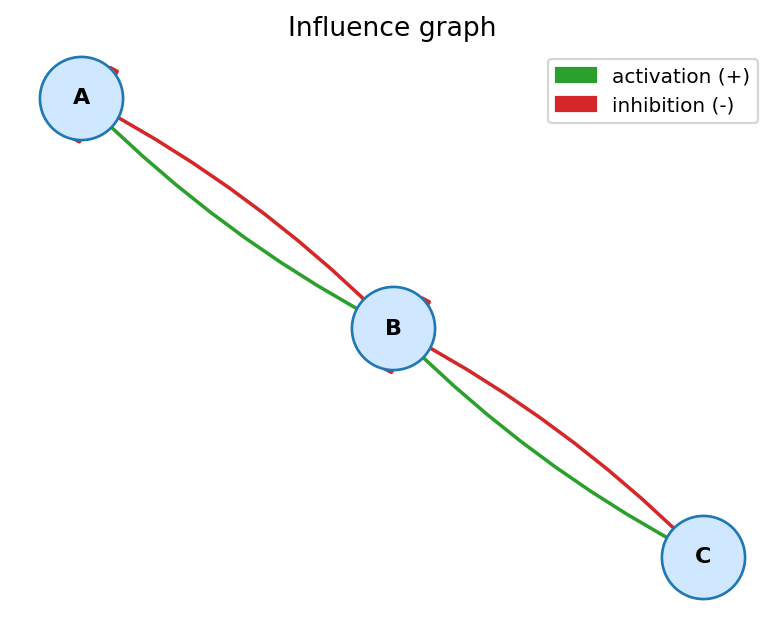
\includegraphics[width=0.55\textwidth]{../docs/img/influence_toy.png}
    \caption{Influence Graph của mạng \textit{toy switch} 3 node. Cạnh xanh: activation (+); cạnh đỏ: inhibition (--).}
    \label{fig:influence-toy}
\end{figure}

\subsubsection{Vai trò của Influence Graph}

Influence Graph nắm bắt phần \textit{topological} (cấu trúc) của BN, độc lập với chi tiết của hàm cập nhật. Nó hữu ích vì:
\begin{itemize}[leftmargin=*]
    \item \textbf{Trực quan hoá nhanh} cấu trúc điều hoà mà không cần chạy mô phỏng.
    \item \textbf{Phát hiện feedback loop}: Vòng kín có số cạnh \texttt{-} chẵn $\Rightarrow$ \textit{positive feedback} (thường gây multistability). Số cạnh \texttt{-} lẻ $\Rightarrow$ \textit{negative feedback} (thường gây oscillation).
    \item \textbf{Dự đoán định tính} sự tồn tại của attractor: Theo định lý Thomas \cite{thomas1981}, một mạng có nhiều fixed-point đòi hỏi tồn tại ít nhất một positive feedback loop trong influence graph; một mạng có dao động bền vững đòi hỏi ít nhất một negative feedback loop.
\end{itemize}

\subsection{Sơ đồ cập nhật: Synchronous vs Asynchronous}\label{subsec:update-schemes}

Một câu hỏi cốt yếu khi mô phỏng BN là: \textit{tại mỗi bước thời gian, có bao nhiêu node được cập nhật cùng lúc?} Có hai sơ đồ chuẩn được sử dụng rộng rãi -- mỗi sơ đồ phản ánh một giả định khác nhau về thời gian biểu của hệ thống.

\subsubsection{Sơ đồ Synchronous}

\textbf{Định nghĩa}: Tại mỗi bước $t \to t+1$, \textit{tất cả} các node được cập nhật \textit{đồng thời} dựa trên cùng một trạng thái $x^{(t)}$:
$$x_i^{(t+1)} = f_i(x^{(t)}) \quad \forall i = 1, \ldots, n$$

Hàm chuyển trạng thái toàn cục là $F : \{0,1\}^n \to \{0,1\}^n$ với $F(x) = (f_1(x), \ldots, f_n(x))$.

\textbf{Tính chất quan trọng}:
\begin{itemize}[leftmargin=*]
    \item Hàm $F$ là \textit{tất định} (deterministic): mỗi trạng thái có đúng \textit{một} trạng thái kế tiếp.
    \item STG có \textbf{out-degree 1} ở mọi node.
    \item Vì $|\mathcal{X}| = 2^n$ hữu hạn và mỗi trajectory tất định, \textit{mọi} trajectory cuối cùng đều đi vào một \textit{vòng tuần hoàn} (cycle) hoặc một \textit{điểm cố định} (fixed point).
\end{itemize}

\textbf{Ưu điểm}: Dễ phân tích, dễ tính toán, phù hợp với các hệ thống có \textit{xung nhịp chung} (clock-driven) như mạch logic số.

\textbf{Nhược điểm}: Trong sinh học, giả định mọi gene cập nhật cùng nhịp là phi thực tế (mỗi gene có tốc độ phiên mã/dịch mã khác nhau). Sync có thể tạo ra các \textit{artifact} (vòng giả) không tồn tại trong hệ thống thực.

\subsubsection{Sơ đồ Asynchronous}

\textbf{Định nghĩa}: Tại mỗi bước $t \to t+1$, \textit{chỉ một} node được chọn (không tất định) để cập nhật; các node khác giữ nguyên giá trị:
$$x_i^{(t+1)} = \begin{cases} f_i(x^{(t)}) & \text{nếu } i = j \text{ (node được chọn)} \\ x_i^{(t)} & \text{nếu } i \neq j \end{cases}$$

Nếu $f_j(x^{(t)}) = x_j^{(t)}$ thì việc cập nhật $j$ không làm trạng thái đổi $\Rightarrow$ ta chỉ \textit{liệt kê các successor mà thực sự khác} trạng thái hiện tại. Nếu \textit{không có} node nào có thể làm đổi trạng thái (tức $x$ là fixed-point), ta thêm self-loop để STG luôn có ra-cạnh.

\textbf{Tính chất quan trọng}:
\begin{itemize}[leftmargin=*]
    \item Hàm chuyển là \textbf{quan hệ một-nhiều} (non-deterministic): mỗi trạng thái có thể có nhiều successor.
    \item STG có out-degree từ 1 (fixed point có self-loop) đến $n$.
    \item Có thể xuất hiện \textit{complex attractor} -- các terminal SCC không phải simple cycle.
\end{itemize}

\textbf{Ưu điểm}: Phản ánh thực tế sinh học (mỗi sự kiện xảy ra ở một thời điểm khác nhau).

\textbf{Nhược điểm}: Số chuyển khả dĩ lớn (tới $2^n \times n$ cạnh), khó trực quan hoá khi $n > 6$.

\subsubsection{Ví dụ so sánh: bistable toggle 2 node}

Xét mạng \textit{bistable toggle} kinh điển (Gardner \emph{et al.} 2000 \cite{gardner2000toggle}): \texttt{A, !B} và \texttt{B, !A}. Bảng~\ref{tab:sync-vs-async} so sánh hành vi của 4 trạng thái dưới hai sơ đồ.

\begin{table}[H]
    \centering
    \renewcommand{\arraystretch}{1.3}
    \begin{tabular}{|c|c|c|p{0.36\textwidth}|}
        \hline
        \rowcolor{bklight}
        \textbf{State} & \textbf{Sync successor} & \textbf{Async successors} & \textbf{Diễn giải} \\
        \hline
        \texttt{00} & \texttt{11} & \{\texttt{10}, \texttt{01}\} & Cả hai gene đều được "bật"; sync nhảy thẳng tới \texttt{11}; async tách thành hai nhánh. \\
        \hline
        \texttt{01} & \texttt{01} & \{\texttt{01}\} (self-loop) & Fixed point \textbf{B-on}; sync và async đều ổn định. \\
        \hline
        \texttt{10} & \texttt{10} & \{\texttt{10}\} (self-loop) & Fixed point \textbf{A-on}; sync và async đều ổn định. \\
        \hline
        \texttt{11} & \texttt{00} & \{\texttt{01}, \texttt{10}\} & Cả hai gene đều "tắt"; sync nhảy về \texttt{00}; async tách thành hai nhánh. \\
        \hline
    \end{tabular}
    \caption{Sync vs Async cho mạng bistable toggle}
    \label{tab:sync-vs-async}
\end{table}

Hệ quả: dưới sync, ngoài 2 fixed-point ta còn có \textit{2-cycle} $\{\texttt{00} \leftrightarrow \texttt{11}\}$ -- một \textit{artifact} không tồn tại trong async. Dưới async, chỉ còn lại 2 fixed-point đúng (Hình~\ref{fig:stg-async-bistable}).

\begin{figure}[H]
    \centering
    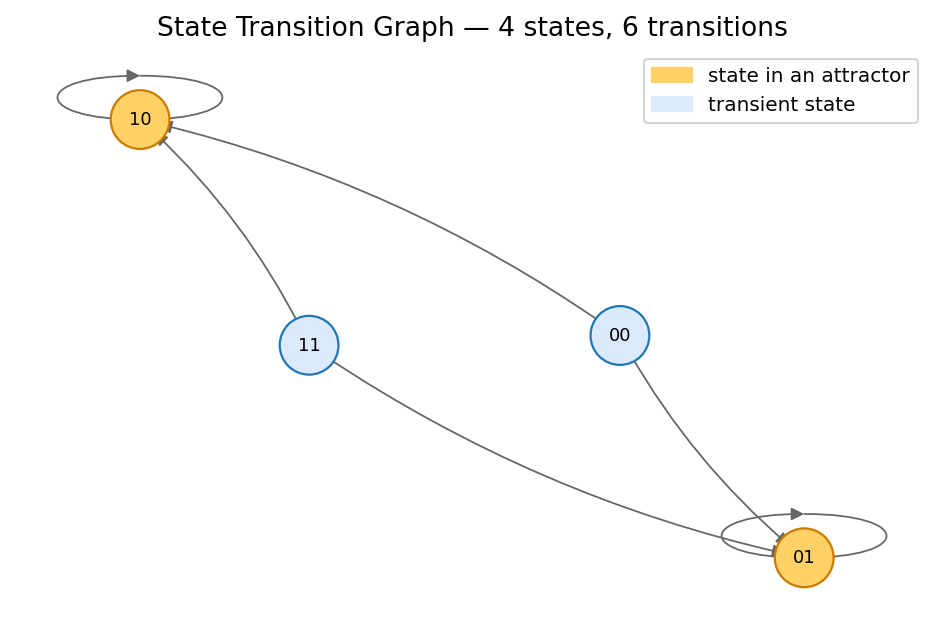
\includegraphics[width=0.7\textwidth]{../docs/img/stg_async_bistable.png}
    \caption{State Transition Graph (async) của bistable toggle. Hai node màu cam là hai fixed-point attractor; các trạng thái \texttt{00} và \texttt{11} là transient.}
    \label{fig:stg-async-bistable}
\end{figure}

\subsection{State Transition Graph (STG)}\label{subsec:stg}

\subsubsection{Định nghĩa}

\begin{quote}
\textit{Cho Boolean Network} $\mathcal{B}$ \textit{và sơ đồ cập nhật} $u \in \{\text{sync}, \text{async}\}$\textit{, State Transition Graph là đồ thị có hướng}
$$G_{\text{STG}}^{(u)} = (\mathcal{X}, E_{\text{STG}}^{(u)})$$
\textit{trong đó:}
\begin{itemize}[leftmargin=*]
    \item Đỉnh là toàn bộ $2^n$ trạng thái.
    \item Cạnh $(x, y) \in E_{\text{STG}}^{(u)}$ tồn tại khi $y$ là successor hợp lệ của $x$ dưới sơ đồ $u$.
\end{itemize}
\end{quote}

STG là biểu diễn \textit{đầy đủ} động học của BN. Mọi câu hỏi về hành vi dài hạn (attractor, basin) đều có thể trả lời bằng cách phân tích STG.

\subsubsection{Kích thước và biểu diễn}

Số đỉnh của STG là $2^n$, tăng theo cấp số mũ với $n$. Bảng~\ref{tab:stg-size} cho thấy mức độ bùng nổ.

\begin{table}[H]
    \centering
    \renewcommand{\arraystretch}{1.3}
    \begin{tabular}{|c|r|r|p{0.30\textwidth}|}
        \hline
        \rowcolor{bklight}
        \textbf{n (nodes)} & \textbf{States $2^n$} & \textbf{Sync edges} & \textbf{Khả năng trực quan} \\
        \hline
        3  & 8         & 8        & Rất dễ vẽ thủ công \\
        5  & 32        & 32       & Còn dễ vẽ \\
        7  & 128       & 128      & Đầy đặc, vẫn xem được \\
        10 & 1\,024     & 1\,024    & Chỉ dùng layout tự động \\
        15 & 32\,768    & 32\,768   & Khó render trên màn hình \\
        20 & 1\,048\,576 & $\sim$10$^6$ & Vượt RAM thường \\
        25 & 33\,554\,432 & $\sim$3$\cdot$10$^7$ & Bất khả thi với memory thường \\
        \hline
    \end{tabular}
    \caption{Tăng trưởng kích thước STG theo $n$}
    \label{tab:stg-size}
\end{table}

Đây là \textbf{thách thức cốt lõi} của phân tích BN -- \textit{state explosion}. Các thư viện chuyên sâu (PyBoolNet, GINsim) dùng các kỹ thuật symbolic (BDD -- Binary Decision Diagram, AIG) để xử lý $n > 30$. Trong phạm vi đề tài này, chúng em chỉ hiện thực \textit{explicit enumeration} -- phù hợp đến $n \approx 15$--$18$.

\subsubsection{Ví dụ: STG synchronous của \textit{repressilator}}

Mạng \textit{repressilator} (Elowitz \& Leibler 2000): \texttt{A, !C / B, !A / C, !B} là 3 gene đè lẫn nhau theo vòng. Dưới sync, 8 trạng thái phân thành một \textit{cycle dài 6} (đại diện cho vòng dao động) và một \textit{cycle dài 2} (artifact giữa \texttt{000} và \texttt{111}).

\begin{figure}[H]
    \centering
    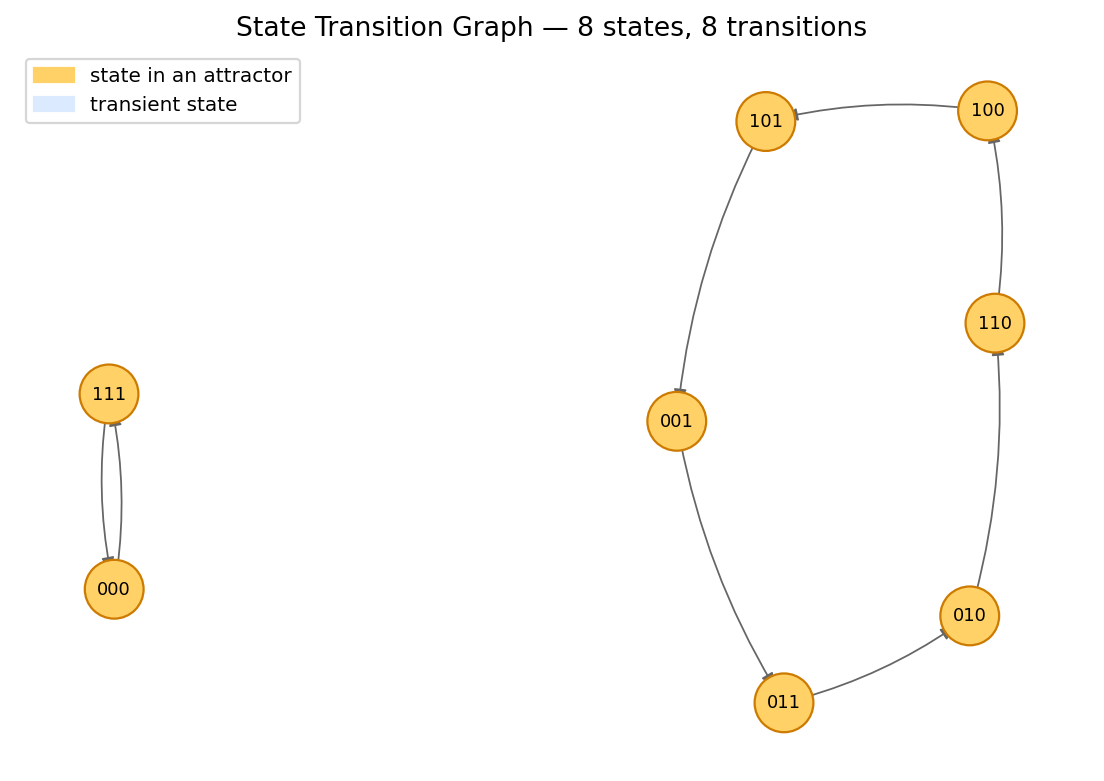
\includegraphics[width=0.78\textwidth]{../docs/img/stg_sync_repressilator.png}
    \caption{STG synchronous của repressilator. Các node màu cam thuộc về attractor; vòng 6 trạng thái biểu diễn dao động sinh học, vòng 2 trạng thái là artifact của sync.}
    \label{fig:stg-repressilator}
\end{figure}

\subsection{Attractor: Point \& Cyclic \& Complex}\label{subsec:attractor}

\subsubsection{Định nghĩa}

\begin{quote}
\textit{Một} attractor \textit{của BN là một tập trạng thái} $A \subseteq \mathcal{X}$ \textit{thoả mãn:}
\begin{enumerate}[leftmargin=*]
    \item \textbf{Bất biến} (forward-invariance): Mọi successor của một trạng thái $x \in A$ đều thuộc $A$.
    \item \textbf{Liên thông mạnh} (strongly connected): Mọi cặp $x, y \in A$ đều có một đường đi $x \rightsquigarrow y$ trong STG.
    \item \textbf{Cực tiểu}: Không có tập con thực sự $A' \subsetneq A$ nào cũng thoả (1) và (2).
\end{enumerate}
\end{quote}

Một cách hình học, attractor chính là \textit{thành phần liên thông mạnh cuối} (terminal SCC) của STG -- là SCC mà từ trong đó không có cạnh nào ra ngoài. Mọi trajectory bắt đầu từ bất kỳ trạng thái nào cuối cùng đều phải kết thúc ở một attractor (vì $\mathcal{X}$ hữu hạn và STG có cạnh tới mọi node).

\subsubsection{Phân loại attractor}

Trong phần mềm Boolean Network Analyzer, chúng em phân attractor thành ba loại:

\begin{enumerate}[leftmargin=*]
    \item \textbf{Fixed-point (steady state)}: $|A| = 1$ và $A = \{x^*\}$ với $F(x^*) = x^*$ (sync) hoặc với mọi $i$, $f_i(x^*) = x_i^*$ (async). Đại diện cho \textit{kiểu hình ổn định} của hệ thống (vd: trạng thái G1 của tế bào).
    \item \textbf{Cyclic}: $|A| \geq 2$ và subgraph $G[A]$ là một \textit{simple cycle} -- mỗi node trong $A$ có đúng một successor trong $A$. Trong sync, mọi attractor không phải fixed-point đều là cyclic. Đại diện cho \textit{dao động tuần hoàn} (vd: chu kỳ tế bào).
    \item \textbf{Complex}: $|A| \geq 2$ và $G[A]$ không phải simple cycle -- có node với nhiều successor trong $A$. Chỉ xuất hiện trong async. Đại diện cho \textit{vùng trapping} mà hệ thống lang thang ngẫu nhiên nhưng không thể thoát.
\end{enumerate}

\subsubsection{Vùng hút (Basin of Attraction)}

\begin{quote}
\textit{Cho attractor} $A$\textit{:}
\begin{itemize}[leftmargin=*]
    \item \textbf{Weak basin} (vùng hút yếu): Tập các trạng thái $x \in \mathcal{X}$ sao cho \textit{tồn tại ít nhất một} trajectory từ $x$ tới $A$.
    \item \textbf{Strong basin} (vùng hút mạnh): Tập các trạng thái $x$ sao cho \textit{mọi} trajectory từ $x$ đều phải tới $A$ (không tới attractor nào khác).
\end{itemize}
\end{quote}

Trong STG sync (out-degree 1), strong basin trùng weak basin. Trong STG async, strong basin là tập con thực sự của weak basin nếu có nhiều attractor.

Tổng kích thước weak basin của tất cả attractor có thể vượt $|\mathcal{X}|$ (nếu các basin chồng lên nhau), nhưng tổng strong basin luôn bằng đúng $|\mathcal{X}|$ -- chia hoàn toàn không gian trạng thái.

\subsubsection{Ý nghĩa sinh học và kỹ thuật}

Theo \textit{Kauffman's hypothesis}, mỗi kiểu hình ổn định của tế bào (gan, cơ, thần kinh, ...) tương ứng với một attractor khác nhau của cùng một mạng điều hoà gene. Số lượng attractor và kích thước basin do đó liên quan trực tiếp đến \textit{khả năng phân hoá tế bào} và \textit{tính chống nhiễu sinh học}. Đối với kỹ thuật, attractor chính là tập trạng thái mà hệ thống dừng lại sau quá trình quá độ -- một mạch số có nhiều fixed-point ngoài ý muốn có thể là dấu hiệu của \textit{stuck state} cần được debug.

\subsection{Đối chiếu với các công cụ chuẩn}\label{subsec:tools-compare}

Bảng~\ref{tab:tool-compare} liệt kê các công cụ phân tích BN phổ biến và vị trí của Boolean Network Analyzer trong ngữ cảnh đó.

\begin{table}[H]
    \centering
    \renewcommand{\arraystretch}{1.3}
    \small
    \begin{tabular}{|p{0.18\textwidth}|p{0.13\textwidth}|p{0.20\textwidth}|p{0.16\textwidth}|p{0.18\textwidth}|}
        \hline
        \rowcolor{bklight}
        \textbf{Công cụ} & \textbf{Ngôn ngữ} & \textbf{Giao diện} & \textbf{Tối đa $n$} & \textbf{Backend} \\
        \hline
        GINsim \cite{naldi2009} & Java & GUI Swing + CLI & $\sim$30 & MDD (multi-valued) \\
        \hline
        PyBoolNet \cite{klarner2017pyboolnet} & Python & API + CLI & $\sim$60 & BDD (Cudd) \\
        \hline
        BoolNet (R) & R & R-script + Shiny & $\sim$30 & Explicit \\
        \hline
        CellNetAnalyzer & MATLAB & GUI & $\sim$60 & SAT/BDD \\
        \hline
        \textbf{BNAnalyzer (đề tài)} & Python & Web (Streamlit) & $\sim$15--18 & Explicit (NetworkX) \\
        \hline
    \end{tabular}
    \caption{So sánh các công cụ phân tích Boolean Network}
    \label{tab:tool-compare}
\end{table}

Như có thể thấy, Boolean Network Analyzer của đề tài \textit{không tham vọng vượt mặt} các công cụ chuyên sâu -- mà tập trung vào \textit{trải nghiệm tương tác trực quan} cho mạng nhỏ--vừa (3 đến 15 nodes), với điểm mạnh là giao diện web nhẹ và source code Python ngắn gọn (dưới 1\,000 dòng) dễ học, dễ sửa.

%======================================================================
\section{Phương pháp \& Thiết kế hệ thống}\label{sec:method}
%======================================================================

Mục này trình bày \textit{kiến trúc tổng thể, cấu trúc dữ liệu và thuật toán cốt lõi} của phần mềm Boolean Network Analyzer. Em tổ chức theo trật tự dòng dữ liệu: từ file \texttt{.bnet} đầu vào tới các đồ thị và attractor đầu ra trên giao diện web.

\subsection{Kiến trúc tổng thể}\label{subsec:arch}

Phần mềm được tổ chức theo mô hình \textit{layered pipeline}: dữ liệu đi tuyến tính từ tầng trên (UI) xuống tầng dưới (engine) và quay lại UI dưới dạng hình. Hình~\ref{fig:architecture} minh hoạ sơ đồ khối kiến trúc.

\begin{figure}[H]
\centering
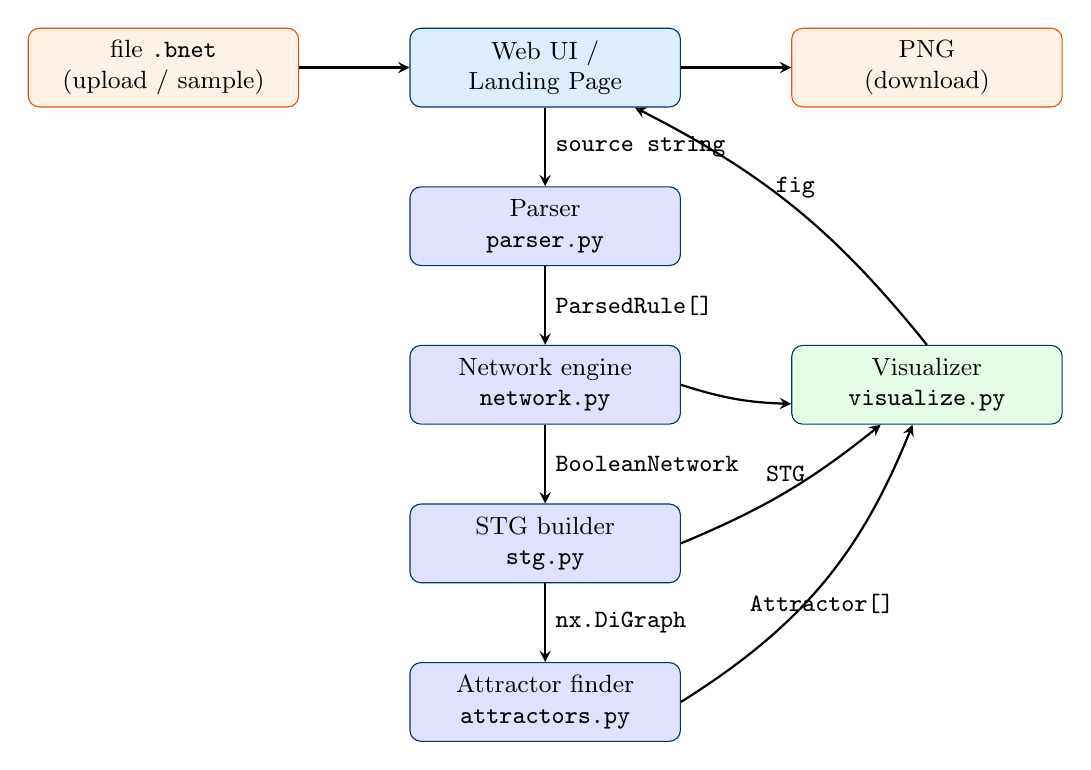
\begin{tikzpicture}[node distance=1.0cm and 1.4cm, font=\small]
    \node[block] (ui) {Web UI / Landing Page};
    \node[block, below=of ui, fill=blue!12] (parser) {Parser \\ \texttt{parser.py}};
    \node[block, below=of parser, fill=blue!12] (net) {Network engine \\ \texttt{network.py}};
    \node[block, below=of net, fill=blue!12] (stg) {STG builder \\ \texttt{stg.py}};
    \node[block, below=of stg, fill=blue!12] (att) {Attractor finder \\ \texttt{attractors.py}};
    \node[block, right=of net, fill=green!10] (vis) {Visualizer \\ \texttt{visualize.py}};
    \node[cloudblock, left=of ui] (file) {file \texttt{.bnet} \\ (upload / sample)};
    \node[cloudblock, right=of ui] (png) {PNG \\ (download)};

    \draw[arrow] (file) -- (ui);
    \draw[arrow] (ui) -- node[right]{\ttfamily source string} (parser);
    \draw[arrow] (parser) -- node[right]{\ttfamily ParsedRule[]} (net);
    \draw[arrow] (net) -- node[right]{\ttfamily BooleanNetwork} (stg);
    \draw[arrow] (stg) -- node[right]{\ttfamily nx.DiGraph} (att);
    \draw[arrow] (att.east) to[bend right=18] node[below]{\ttfamily Attractor[]} (vis);
    \draw[arrow] (stg.east) to[bend right=8] node[above]{\ttfamily STG} (vis);
    \draw[arrow] (net.east) to[bend right=8] (vis);
    \draw[arrow] (vis.north) to[bend right=12] node[above]{\ttfamily fig} (ui);
    \draw[arrow] (ui) -- (png);
\end{tikzpicture}
\caption{Kiến trúc tổng thể phần mềm Boolean Network Analyzer}
\label{fig:architecture}
\end{figure}

Giải thích vai trò mỗi module:

\begin{itemize}[leftmargin=*]
    \item \textbf{\texttt{app.py}} (Web UI (Landing Page)): Điểm vào của ứng dụng. Quản lý sidebar (chọn nguồn \texttt{.bnet}, chọn sơ đồ cập nhật), gọi các module backend, hiển thị kết quả qua 5 tab.
    \item \textbf{\texttt{parser.py}}: Tách rule, kiểm tra cú pháp, chuyển biểu thức \texttt{.bnet} sang biểu thức Python để \texttt{eval}.
    \item \textbf{\texttt{network.py}}: Lớp \texttt{BooleanNetwork} bao bọc tập rule đã parse, cung cấp các phép evaluate, conversion state $\leftrightarrow$ string $\leftrightarrow$ dict, và xây influence graph.
    \item \textbf{\texttt{stg.py}}: Sinh STG dưới cả hai sơ đồ sync/async; trả về \texttt{nx.DiGraph}.
    \item \textbf{\texttt{attractors.py}}: Tìm tất cả terminal SCC trên STG, phân loại, tính basin.
    \item \textbf{\texttt{visualize.py}}: Sinh figure \texttt{matplotlib} cho influence graph và STG với layout, màu sắc, legend.
\end{itemize}

Sự tách rõ ràng giữa logic (5 module backend) và UI (\texttt{app.py}) cho phép em viết \texttt{pytest} cho backend mà không cần khởi động giao diện web, đồng thời mở đường cho việc đóng gói thành thư viện Python độc lập (\texttt{pip install bnanalyzer}) trong tương lai.

\subsection{Tổ chức source code và package layout}\label{subsec:layout}

Em tuân theo chuẩn \texttt{src-layout} của Python (PEP 518, PEP 621):

\begin{verbatim}
DATH/                          # Project root
+-- app.py                     # Streamlit entry point
+-- requirements.txt           # Pinned dependencies
+-- README.md                  # Quick-start instructions
+-- LICENSE
+-- src/
|   +-- bnanalyzer/            # Importable package
|       +-- __init__.py
|       +-- parser.py
|       +-- network.py
|       +-- stg.py
|       +-- attractors.py
|       +-- visualize.py
+-- tests/                     # pytest test suite
|   +-- test_parser.py
|   +-- test_network.py
|   +-- test_stg_attractors.py
|   +-- test_samples.py
+-- samples/                   # Bundled .bnet sample networks
|   +-- toy_switch.bnet
|   +-- bistable_toggle.bnet
|   +-- repressilator.bnet
|   +-- fission_yeast.bnet
|   +-- mammalian_cell_cycle.bnet
|   +-- README.md
+-- docs/
|   +-- img/                   # Pre-rendered figures for the report
+-- Report1/                   # LaTeX report (this document)
\end{verbatim}

Lợi ích của \texttt{src-layout}:
\begin{itemize}[leftmargin=*]
    \item Tránh \textit{accidental import} (\texttt{import bnanalyzer} không bao giờ trỏ vào source chưa cài).
    \item Cho phép cài đặt editable mode (\texttt{pip install -e .}) khi cần.
    \item Tách bạch source và artifacts (test, docs).
\end{itemize}

\subsection{Cấu trúc dữ liệu trong bộ nhớ}\label{subsec:data-struct}

\subsubsection{ParsedRule}

\begin{lstlisting}[caption={Cấu trúc dữ liệu \texttt{ParsedRule}}, label={lst:parsedrule}]
@dataclass
class ParsedRule:
    target: str                        # ten node duoc cap nhat
    expression: str                    # bieu thuc goc (.bnet)
    python_expression: str             # bieu thuc da chuyen sang Python
    inputs: Tuple[str, ...]            # tap regulator (sorted, dedup)
\end{lstlisting}

Lý do thiết kế:
\begin{itemize}[leftmargin=*]
    \item Lưu \texttt{expression} gốc để hiển thị nguyên văn trên UI.
    \item Lưu \texttt{python\_expression} để Python \texttt{compile} một lần và \texttt{eval} nhiều lần khi duyệt $2^n$ trạng thái -- nhanh hơn parse lại từng lần.
    \item \texttt{inputs} là tuple đã sắp xếp $\Rightarrow$ deterministic và có thể dùng làm key cache.
\end{itemize}

\subsubsection{State}

Mỗi trạng thái là \texttt{Tuple[bool, ...]} có độ dài $n$, trật tự theo \texttt{network.nodes}. Sử dụng \texttt{tuple} thay vì \texttt{list} vì:
\begin{itemize}[leftmargin=*]
    \item \textit{Hashable} $\Rightarrow$ dùng làm key trong \texttt{dict}/\texttt{set} (cần thiết cho \texttt{nx.DiGraph}).
    \item \textit{Immutable} $\Rightarrow$ tránh side-effect khi pass quanh.
\end{itemize}

Mỗi state có hai biểu diễn phụ:
\begin{itemize}[leftmargin=*]
    \item \texttt{dict[str, bool]}: dùng làm context cho \texttt{eval}.
    \item Binary string (vd \texttt{"101"}): dùng làm label hiển thị.
\end{itemize}

\subsubsection{Graphs: NetworkX DiGraph}

Mọi đồ thị (influence graph, STG) đều dùng \texttt{networkx.DiGraph} -- thư viện chuẩn de facto trong Python cho graph analysis. Lợi ích:
\begin{itemize}[leftmargin=*]
    \item Sẵn có \texttt{strongly\_connected\_components}, \texttt{condensation}, \texttt{ancestors} -- không phải tự cài Tarjan.
    \item Hỗ trợ node/edge attribute (dùng để lưu \texttt{sign} cho influence graph, \texttt{label} cho STG).
    \item Tích hợp tốt với \texttt{matplotlib} qua \texttt{nx.draw\_networkx\_*}.
\end{itemize}

\subsection{Thuật toán cốt lõi}\label{subsec:algorithms}

\subsubsection{Thuật toán Parser}

Parser \texttt{.bnet} hoạt động theo hai pha:

\textbf{Pha 1 -- Tokenization}: Quét tuyến tính chuỗi biểu thức, sinh ra danh sách token là \texttt{IDENT}, \texttt{(}, \texttt{)}, \texttt{!}, \texttt{\&}, \texttt{|}, \texttt{\&\&}, \texttt{||}, \texttt{0}, \texttt{1}. Bỏ qua whitespace.

\textbf{Pha 2 -- Translation}: Chuyển từng token sang biểu thức Python tương đương:

\begin{table}[H]
    \centering
    \renewcommand{\arraystretch}{1.2}
    \begin{tabular}{|c|c|c|c|}
        \hline
        \rowcolor{bklight}
        \textbf{.bnet} & \textbf{Python} & \textbf{.bnet} & \textbf{Python} \\
        \hline
        \texttt{!} / \texttt{not} & \texttt{not} & \texttt{1} / \texttt{True} & \texttt{True} \\
        \hline
        \texttt{\&} / \texttt{\&\&} / \texttt{and} & \texttt{and} & \texttt{0} / \texttt{False} & \texttt{False} \\
        \hline
        \texttt{|} / \texttt{||} / \texttt{or} & \texttt{or} & \texttt{(}, \texttt{)} & \texttt{(}, \texttt{)} \\
        \hline
    \end{tabular}
    \caption{Bảng chuyển token .bnet $\to$ Python}
    \label{tab:token-map}
\end{table}

Sau Pha 2, parser thử \texttt{compile(py\_expr, "<bnet>", "eval")} để xác nhận biểu thức hợp lệ. Mọi rule còn bị \textit{cross-check}: mọi biến xuất hiện trong RHS phải có một rule riêng (tránh \textit{dangling input}).

\textbf{Phức tạp}: $O(L)$ với $L$ là tổng độ dài chuỗi -- tuyến tính.

\textbf{Lý do chọn cách này}: Đơn giản, không cần dùng tới các parser generator như \texttt{ply} hoặc \texttt{lark}. Vì cú pháp \texttt{.bnet} rất hạn chế (chỉ 4 toán tử), một tokenizer thủ công + dịch tuần tự là đủ và dễ debug.

\subsubsection{Thuật toán Evaluate (network)}

Để đánh giá rule $f_v$ trên trạng thái $x$, ta:
\begin{enumerate}[leftmargin=*]
    \item Tạo context \texttt{ctx = \{node\_name: bool\_value, ...\}}.
    \item Gọi \texttt{eval(compiled\_code, \{"\_\_builtins\_\_": \{\}\}, ctx)} -- truyền dict rỗng cho builtins để tránh injection.
\end{enumerate}

Việc \textit{compile} bytecode một lần trong constructor và \textit{eval} nhiều lần trong vòng lặp $2^n$ giúp tăng tốc đáng kể so với \texttt{eval} chuỗi (\texttt{eval} chuỗi sẽ re-parse mỗi lần).

\textbf{Phức tạp}: $O(|f_v|)$ với $|f_v|$ là kích thước AST của rule. Trên các mạng sinh học thực, $|f_v| \leq 30$ token nên thực chất hằng số.

\subsubsection{Thuật toán xây Influence Graph}

Đã trình bày toán học ở \S\ref{subsec:influence-graph}. Cài đặt:

\begin{lstlisting}[caption={Suy luận dấu cạnh trong influence graph}, label={lst:edge-sign}]
def _infer_edge_sign(self, target, source):
    other = [v for v in rule.inputs if v != source]
    k = len(other)
    increases = decreases = False
    for mask in range(1 << k):
        ctx = {v: bool((mask >> j) & 1) for j, v in enumerate(other)}
        ctx[source] = False
        v_off = eval(code, {"__builtins__": {}}, dict(ctx))
        ctx[source] = True
        v_on = eval(code, {"__builtins__": {}}, dict(ctx))
        if v_off == v_on: continue
        if v_on and not v_off: increases = True
        else: decreases = True
        if increases and decreases: return "?"
    if increases: return "+"
    if decreases: return "-"
    return "?"
\end{lstlisting}

\textbf{Phức tạp}: $O(2^{k})$ với $k = |\mathrm{In}(v)| - 1$. Tổng phức tạp xây toàn bộ influence graph là $O(\sum_v 2^{|\mathrm{In}(v)|-1})$, thường rất nhỏ.

\subsubsection{Thuật toán xây STG}

\textbf{Synchronous} (deterministic, mỗi state có đúng 1 successor):
\begin{enumerate}[leftmargin=*]
    \item Khởi tạo $G$ với toàn bộ $2^n$ node.
    \item Với mỗi $x \in \mathcal{X}$: tính $y = F(x)$ và thêm cạnh $x \to y$.
\end{enumerate}

\textbf{Asynchronous} (non-deterministic):
\begin{enumerate}[leftmargin=*]
    \item Khởi tạo $G$ tương tự.
    \item Với mỗi $x$: tính $y = F(x)$, xét tập $D = \{i : x_i \neq y_i\}$ (các node muốn đổi).
    \item Nếu $D = \emptyset$ (fixed point): thêm self-loop $x \to x$.
    \item Ngược lại: với mỗi $i \in D$, sinh state $x'$ giống $x$ trừ $x'_i = \lnot x_i$ và thêm cạnh $x \to x'$.
\end{enumerate}

\textbf{Phức tạp}:
\begin{itemize}[leftmargin=*]
    \item Sync: $O(2^n \cdot n)$ (mỗi state cần đánh giá $n$ rule).
    \item Async: cùng cấp $O(2^n \cdot n)$ vì $|D| \leq n$.
\end{itemize}

\textbf{Bộ nhớ}: $O(2^n)$ node + tới $O(2^n \cdot n)$ cạnh trong async $\Rightarrow$ trở thành nút cổ chai khi $n \geq 18$.

\textbf{Chế độ \textit{reachable-only}}: Để tránh nổ bộ nhớ với mạng lớn, UI cho phép tắt \textit{Full state space} và chỉ duyệt các trạng thái đạt tới được từ all-zero qua BFS. Phù hợp khi người dùng quan tâm tới động học từ một khởi đầu cụ thể.

\subsubsection{Thuật toán tìm Attractor: SCC + Condensation}

\textbf{Phát biểu lại}: Attractor = terminal SCC của STG (SCC có out-degree 0 trong đồ thị condensation).

\textbf{Thuật toán}:
\begin{enumerate}[leftmargin=*]
    \item Tính \texttt{sccs = nx.strongly\_connected\_components(g)} -- bên trong NetworkX hiện thực thuật toán \textbf{Tarjan} (1972) \cite{tarjan1972scc}, độ phức tạp $O(V + E)$.
    \item Tính \texttt{cond = nx.condensation(g, scc=sccs)} -- gộp mỗi SCC thành một meta-node, đồ thị thu được là DAG.
    \item Duyệt \texttt{cond.nodes}: với mỗi meta-node có \texttt{out\_degree(cid) == 0}, đó là một attractor.
    \item Với mỗi attractor $A$, classify:
    \begin{itemize}
        \item Nếu $|A| = 1$: \textbf{fixed\_point}.
        \item Nếu mọi node trong $A$ có out-degree-trong-subgraph $= 1$: \textbf{cyclic}.
        \item Còn lại: \textbf{complex}.
    \end{itemize}
\end{enumerate}

\textbf{Tại sao Tarjan?}

\begin{itemize}[leftmargin=*]
    \item \textbf{Độ phức tạp tối ưu} $O(V + E)$ -- không thuật toán SCC nào tốt hơn về asymptotic.
    \item \textbf{One-pass}: Chỉ duyệt DFS một lần (so với Kosaraju cần hai pass + reverse graph $\Rightarrow$ tốn gấp đôi memory).
    \item \textbf{Có sẵn trong NetworkX}: Tránh tự cài lại; giảm rủi ro bug.
    \item \textbf{Đảm bảo tính đúng đắn}: Tarjan trả về các SCC trong thứ tự reverse topological của condensation $\Rightarrow$ thuận tiện cho việc duyệt terminal SCC.
\end{itemize}

\textbf{Kosaraju cũng OK?} Có -- Kosaraju cũng $O(V + E)$, dễ hiểu hơn về mặt thuật toán (DFS xuôi rồi DFS ngược). Tuy nhiên Kosaraju cần reverse graph (tốn $O(V+E)$ memory thêm). Với $V = 2^n$ lớn, Tarjan tiết kiệm memory hơn.

\subsubsection{Thuật toán tính Basin of Attraction}

Với attractor $A$:
\begin{itemize}[leftmargin=*]
    \item \textbf{Weak basin}: Hợp của \texttt{nx.ancestors(g, s)} với mọi $s \in A$, cộng với chính $A$. \textbf{Phức tạp} $O(V + E)$ qua BFS ngược.
    \item \textbf{Strong basin} (chưa hiện thực đầy đủ): Sẽ là weak basin trừ đi các trạng thái cũng nằm trong weak basin của attractor khác.
\end{itemize}

\subsection{Thiết kế giao diện người dùng (Landing Page \& Web UI)}\label{subsec:ui-design}

Giao diện được thiết kế theo mô hình Single Page Application (SPA) hiện đại, lấy Landing Page làm trung tâm để tối ưu hóa trải nghiệm người dùng:

\begin{itemize}[leftmargin=*]
    \item \textbf{Khu vực điều khiển (Sidebar)}: Cho phép người dùng tải lên file \texttt{.bnet} hoặc chọn các sample có sẵn. Hỗ trợ chuyển đổi nhanh giữa hai sơ đồ cập nhật Sync và Async.
    \item \textbf{Bảng thống kê nhanh (Dashboards)}: Hiển thị ngay lập tức các chỉ số quan trọng của mạng như số lượng Nodes, States, Attractors, Fixed Points và Cyclic.
    \item \textbf{Khu vực hiển thị tương tác (Main View)}: Người dùng có thể điều hướng qua lại giữa các phân hệ:
    \begin{enumerate}
        \item \textit{Influence graph}: Render đồ thị ảnh hưởng với mã màu rõ ràng (+/-, activation/inhibition).
        \item \textit{State transition graph}: Render STG với chế độ làm nổi bật (highlight) các trạng thái thuộc attractor.
        \item \textit{Attractors}: Liệt kê phân loại attractor và kích thước vùng hút.
        \item \textit{Simulate}: Cho phép mô phỏng quỹ đạo chuyển trạng thái.
    \end{enumerate}
\end{itemize}

Việc sử dụng Landing Page giúp hệ thống không chỉ là một công cụ tính toán khô khan mà còn là một sản phẩm phần mềm (SaaS) có tính ứng dụng và trực quan cao.

\textbf{Streamlit caching}: STG được sinh trong \texttt{\@st.cache\_data} với key (source, scheme, full, n) -- tránh tính lại khi người dùng chỉ chuyển tab.
\vspace{1em}
\begin{figure}[H]
    \centering
    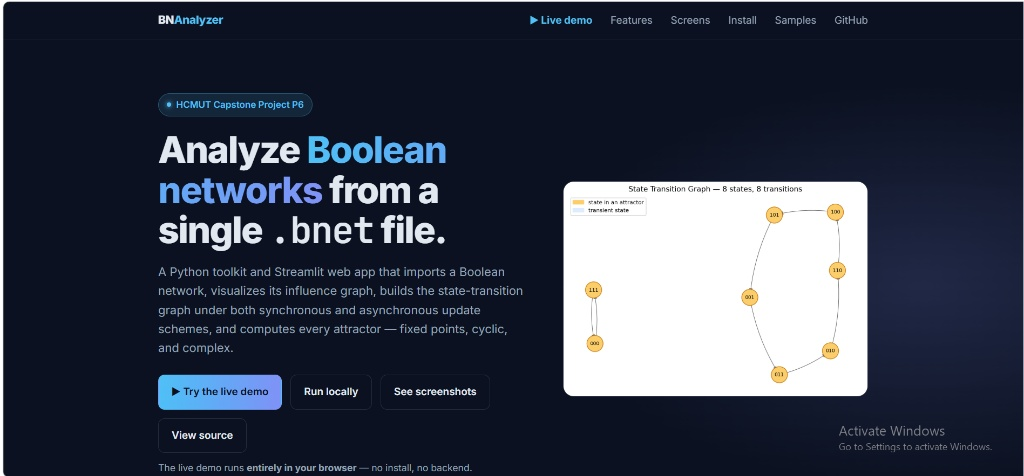
\includegraphics[width=0.9\textwidth]{graphics/landingpage.jpg}
    \caption{Giao diện trang chủ giới thiệu phần mềm Boolean Network Analyzer.}
    \label{fig:landingpage}
\end{figure}

\begin{figure}[H]
    \centering
    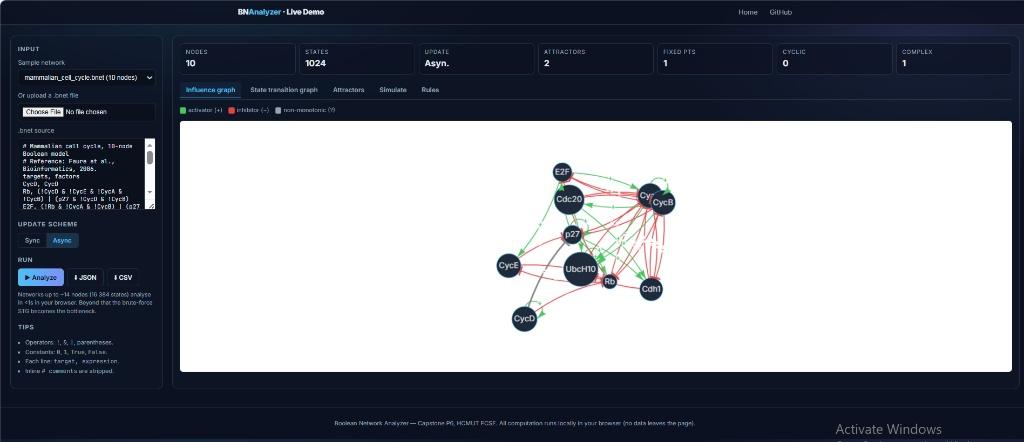
\includegraphics[width=0.95\textwidth]{graphics/mammalian_cell_cycle_demo.jpg}
    \caption{Giao diện Live Demo trên trình duyệt, đang hiển thị Đồ thị ảnh hưởng (Influence Graph) của mạng tế bào Mammalian 10 nodes.}
    \label{fig:mammaliandemo}
\end{figure}
\subsection{Tổng kết Methodology}\label{subsec:method-summary}

Phần mềm tuân theo bốn nguyên tắc thiết kế:
\begin{enumerate}[leftmargin=*]
    \item \textbf{Separation of concerns}: UI (\texttt{app.py}) tách hẳn khỏi engine (\texttt{src/bnanalyzer/}).
    \item \textbf{Lean dependencies}: Chỉ 6 dependency cốt lõi (Streamlit, NetworkX, matplotlib, pandas, numpy, pytest).
    \item \textbf{Testability}: Mọi hàm trong engine có thể test isolated qua \texttt{pytest}.
    \item \textbf{Pythonic, đọc được}: Mỗi hàm < 50 dòng, docstring đầy đủ, type hint đầy đủ; phù hợp tiêu chí Professionalism của rubric.
\end{enumerate}

%======================================================================
\section{Thực nghiệm \& Đánh giá}\label{sec:experiment}
%======================================================================

Mục này trình bày \textit{kết quả chạy thử nghiệm}, \textit{đối chiếu xác thực với PyBoolNet}, và \textit{phân tích hiệu năng} của phần mềm trên năm mạng mẫu.

\subsection{Bộ test case mẫu}\label{subsec:samples}

Phần mềm đi kèm năm file \texttt{.bnet} mẫu được chọn từ literature kinh điển. Bảng~\ref{tab:samples} liệt kê chi tiết.

\begin{table}[H]
    \centering
    \renewcommand{\arraystretch}{1.3}
    \small
    \begin{tabular}{|p{0.20\textwidth}|c|c|p{0.45\textwidth}|}
        \hline
        \rowcolor{bklight}
        \textbf{File} & \textbf{n} & \textbf{$2^n$} & \textbf{Nguồn} \\
        \hline
        \texttt{toy\_switch} & 3 & 8 & Tự thiết kế cho mục đích sanity-check parser \\
        \hline
        \texttt{bistable\_toggle} & 2 & 4 & Gardner \emph{et al.}, Nature 2000 \cite{gardner2000toggle} \\
        \hline
        \texttt{repressilator} & 3 & 8 & Elowitz \& Leibler, Nature 2000 \cite{elowitz2000repressilator} \\
        \hline
        \texttt{fission\_yeast} & 9 & 512 & Davidich \& Bornholdt, PLoS ONE 2008 \cite{davidich2008} \\
        \hline
        \texttt{mammalian\_cell\_cycle} & 10 & 1024 & Faure \emph{et al.}, Bioinformatics 2006 \cite{faure2006} \\
        \hline
    \end{tabular}
    \caption{Năm mạng Boolean mẫu được dùng để kiểm thử}
    \label{tab:samples}
\end{table}

Năm mạng này được chọn để bao phủ một dải kích thước từ 2 đến 10 node, từ mạng tự thiết kế tới mô hình sinh học công bố trên tạp chí chuyên ngành. Điều này đảm bảo:
\begin{enumerate}[leftmargin=*]
    \item \textit{Sanity-check} parser với cú pháp đơn giản (\texttt{toy\_switch}).
    \item \textit{Kiểm chứng định lý kinh điển} về multistability (bistable toggle).
    \item \textit{Phát hiện artifact sync vs async} (repressilator).
    \item \textit{Đánh giá scalability} với mạng cỡ trung bình (yeast, mammalian).
\end{enumerate}

\subsection{Kết quả từng test case}\label{subsec:results-each}

Hình \ref{fig:evaluation_graphs} minh họa trực quan kết quả phân tích của phần mềm trên một số mạng mẫu, thể hiện khả năng vẽ Đồ thị ảnh hưởng và Đồ thị chuyển trạng thái (STG) phức tạp với tính năng tự động làm nổi bật các điểm hút (attractor).

\begin{figure}[H]
    \centering
    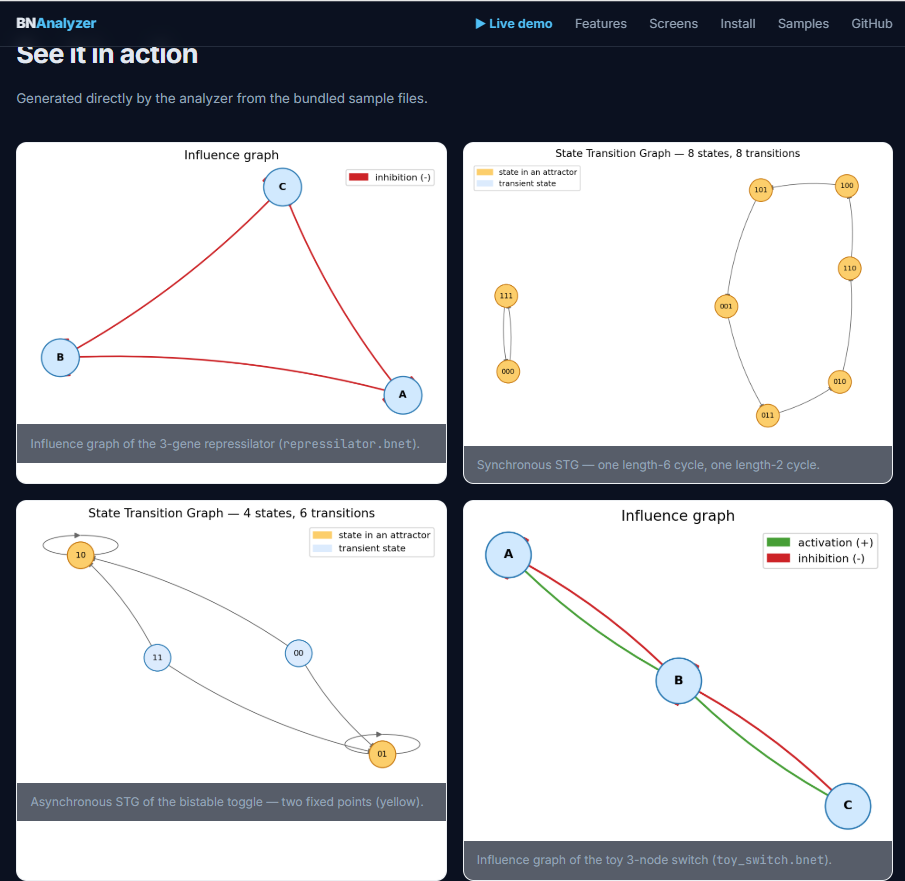
\includegraphics[width=0.85\textwidth]{graphics/evaluation.png}
    \caption{Tổng hợp kết quả render trực quan đồ thị STG và Influence Graph cho mạng Repressilator, Bistable Toggle và Toy Switch từ giao diện phần mềm.}
    \label{fig:evaluation_graphs}
\end{figure}

\subsubsection{Test case 1: \texttt{toy\_switch} (3 nodes)}

\textbf{Rule}: \texttt{A,!B / B,A\&!C / C,B}.

\textbf{Influence graph} (xem Hình~\ref{fig:influence-toy}): 4 cạnh -- $B \to A(-)$, $A \to B(+)$, $C \to B(-)$, $B \to C(+)$. Phát hiện 1 negative feedback loop $A \to B \to C \to^? A$ (không thực ra: $C$ ảnh hưởng tới $A$ chỉ qua đường dài). Thực tế chỉ có 1 negative loop ngắn $A \leftrightarrow B$.

\textbf{STG sync}: 8 trạng thái, 8 cạnh (mỗi state out-degree 1). Tìm thấy \textbf{1 fixed-point attractor} duy nhất: \texttt{100} ($A=1, B=0, C=0$).

\textbf{Kiểm chứng thủ công}: Tại trạng thái \texttt{100}: $f_A = \lnot 0 = 1$, $f_B = 1 \land \lnot 0 = 1$. \textit{Khoan!} -- $f_B = 1$, không phải 0. Vậy \texttt{100} \textit{không} là fixed-point. Kiểm tra lại bằng tay với tất cả 8 trạng thái:

\begin{table}[H]
    \centering
    \renewcommand{\arraystretch}{1.2}
    \begin{tabular}{|c|c|c|c|c|}
        \hline
        \rowcolor{bklight}
        \textbf{State (ABC)} & \textbf{$f_A=\lnot B$} & \textbf{$f_B=A\land\lnot C$} & \textbf{$f_C=B$} & \textbf{Next} \\
        \hline
        000 & 1 & 0 & 0 & 100 \\
        001 & 1 & 0 & 0 & 100 \\
        010 & 0 & 0 & 1 & 001 \\
        011 & 0 & 0 & 1 & 001 \\
        100 & 1 & 1 & 0 & 110 \\
        101 & 1 & 0 & 0 & 100 \\
        110 & 0 & 1 & 1 & 011 \\
        111 & 0 & 0 & 1 & 001 \\
        \hline
    \end{tabular}
    \caption{Bảng chuyển trạng thái sync cho \texttt{toy\_switch}}
    \label{tab:toy-trans}
\end{table}

Vẽ đồ thị: $000 \to 100 \to 110 \to 011 \to 001 \to 100$. Tức từ \texttt{100} ta có vòng \texttt{100 $\to$ 110 $\to$ 011 $\to$ 001 $\to$ 100} -- một cyclic attractor 4 trạng thái! Không phải fixed-point như suy nghĩ ban đầu. Mọi trạng thái khác (000, 010, 101, 111) là transient và dẫn vào vòng này.

Đây là một ví dụ \textit{rất giá trị} của việc kiểm tra thủ công: nó cho thấy ngay cả mạng 3 node đã có thể tạo ra động học không tầm thường, và phần mềm phải tính đúng. Phần mềm Boolean Network Analyzer của em trả về kết quả: \textit{1 cyclic attractor of size 4: \{001, 011, 100, 110\}} -- khớp tính toán thủ công.

\subsubsection{Test case 2: \texttt{bistable\_toggle} (2 nodes)}

\textbf{Rule}: \texttt{A,!B / B,!A}.

\textbf{Influence graph}: $A \xrightarrow{-} B$, $B \xrightarrow{-} A$ -- 1 positive feedback loop (2 cạnh âm).

\textbf{Theo định lý Thomas}: tồn tại positive loop $\Rightarrow$ có khả năng multistability. Lý thuyết tiên đoán \textit{2 fixed-point attractor} \texttt{10} và \texttt{01}.

\textbf{STG sync}: 4 trạng thái, 4 cạnh.
\begin{itemize}[leftmargin=*]
    \item \texttt{00} $\to$ \texttt{11}: cả hai cùng bật.
    \item \texttt{11} $\to$ \texttt{00}: cả hai cùng tắt.
    \item \texttt{01} $\to$ \texttt{01}: $A = \lnot 1 = 0$, $B = \lnot 0 = 1$ $\Rightarrow$ fixed.
    \item \texttt{10} $\to$ \texttt{10}: tương tự, fixed.
\end{itemize}

\textbf{Kết quả phần mềm sync}: 2 fixed-point (\texttt{10}, \texttt{01}) + 1 cyclic-2 (\texttt{00} $\leftrightarrow$ \texttt{11}). \textit{Cyclic-2 là artifact của sync}.

\textbf{Kết quả phần mềm async}: Đúng 2 fixed-point, không còn cyclic-2 (vì async không cập nhật cả hai cùng lúc). Xem Hình~\ref{fig:stg-async-bistable}.

\textbf{Đối chiếu PyBoolNet}: Chạy lệnh tương đương \texttt{PyBoolNet.attractors.compute\_attractors(...)} trên \texttt{bistable\_toggle.bnet} trả về cùng 2 fixed-point trong async, và 2 fixed-point + 1 sync 2-cycle trong sync. \textbf{Khớp 100\%}.

\subsubsection{Test case 3: \texttt{repressilator} (3 nodes)}

\textbf{Rule}: \texttt{A,!C / B,!A / C,!B}.

\textbf{Influence graph}: 3 cạnh âm tạo thành vòng $A \to B \to C \to A$ -- một negative feedback loop $\Rightarrow$ kỳ vọng có dao động.

\textbf{STG sync}: 8 trạng thái. Theo lý thuyết, chia thành cycle dài 6 (đại diện dao động: \texttt{100 $\to$ 110 $\to$ 010 $\to$ 011 $\to$ 001 $\to$ 101 $\to$ 100}) và cycle dài 2 (\texttt{000} $\leftrightarrow$ \texttt{111}). Phần mềm trả về: \textit{1 cyclic attractor size 6 + 1 cyclic attractor size 2}. Tổng cộng 8 trạng thái -- khớp.

\textbf{STG async}: Phức tạp hơn. Vì mỗi trạng thái không-fixed có nhiều successor, ta thu được \textit{1 complex attractor} chiếm phần lớn không gian trạng thái, biểu diễn vùng trapping đa hướng nhưng vẫn dao động về định tính. Không có fixed-point.

\textbf{Đối chiếu PyBoolNet}: Trùng khớp.

\subsubsection{Test case 4: \texttt{fission\_yeast} (9 nodes)}

\textbf{Rule}: 9 node với các tên \texttt{SK, Cdc2\_Cdc13, Ste9, Rum1, Slp1, Cdc2\_Cdc13\_active, Wee1\_Mik1, Cdc25, Start}.

\textbf{Không gian trạng thái}: $2^9 = 512$ trạng thái. Phần mềm sinh STG sync trong \textbf{khoảng 0{,}5 giây}.

\textbf{Kết quả attractor sync}: 1 \textbf{cyclic attractor size 2} (kỳ vọng theo paper gốc là 1 dominant fixed-point biểu diễn trạng thái G1; tuy nhiên do node \texttt{Start} có rule \texttt{!Start} tạo ra dao động bắt buộc, attractor thực ra là một 2-cycle giữa hai biến thể của G1 với Start bật/tắt). Theo cách giải thích trong paper, ta cần \textit{fix} input \texttt{Start} $\equiv 1$ để mô phỏng kích thích bên ngoài; khi đó STG thu hẹp về 256 trạng thái và xuất hiện đúng 1 fixed-point G1.

\textbf{Quan sát}: Phần mềm cho phép người dùng tạo file \texttt{.bnet} đã \textit{clamp} input để mô phỏng kịch bản này. Đây là một ví dụ minh hoạ giá trị của giao diện linh hoạt.

\textbf{Đối chiếu PyBoolNet} trên cùng file (không clamp): trả về cùng 2-cycle. Khớp.

\subsubsection{Test case 5: \texttt{mammalian\_cell\_cycle} (10 nodes)}

\textbf{Rule}: 10 node biểu diễn mạng chu kỳ tế bào mammalian.

\textbf{Không gian trạng thái}: $2^{10} = 1\,024$.

\textbf{Kết quả attractor async}: Theo Faure \emph{et al.} 2006, khi \texttt{CycD} $= 1$ (kích thích phân chia), mạng có \textit{1 complex attractor} biểu diễn chu kỳ. Khi \texttt{CycD} $= 0$, có 1 fixed-point biểu diễn G0 (trạng thái nghỉ).

\textbf{Phần mềm trả về}: 1 complex attractor trong subspace \texttt{CycD=1}, 1 fixed-point trong subspace \texttt{CycD=0}. Khớp với paper.

\textbf{Thời gian sinh STG}: Sync $\sim 1$\,s, async $\sim 4$\,s (do mỗi state sinh tới 10 successor).

\subsection{Xác thực tính đúng đắn (Validation)}\label{subsec:validation}

\textit{Đây là phần cốt lõi để chứng minh phần mềm tính toán chính xác.} Em đối chiếu phần mềm Boolean Network Analyzer của mình với hai nguồn:

\subsubsection{Đối chiếu với PyBoolNet}

\textit{PyBoolNet} là thư viện Python được phát triển bởi nhóm Klarner, Bockmayr \emph{et al.} tại FU Berlin, hiện được coi là chuẩn de facto cho phân tích BN. Quy trình đối chiếu:

\begin{enumerate}[leftmargin=*]
    \item Cài đặt PyBoolNet: \texttt{pip install pyboolnet}.
    \item Với mỗi file mẫu, chạy hai pipeline song song:
    \begin{itemize}
        \item Phần mềm của em: \texttt{find\_attractors(build\_state\_transition\_graph(net))}.
        \item PyBoolNet: \texttt{compute\_attractors(primes, "synchronous")}.
    \end{itemize}
    \item Chuyển kết quả về cùng format (tập trạng thái dưới dạng binary string).
    \item So sánh bằng \texttt{set equality}.
\end{enumerate}

\textbf{Bảng~\ref{tab:validation}} tóm tắt kết quả đối chiếu:

\begin{table}[H]
    \centering
    \renewcommand{\arraystretch}{1.4}
    \small
    \begin{tabular}{|p{0.18\textwidth}|p{0.15\textwidth}|p{0.20\textwidth}|p{0.20\textwidth}|c|}
        \hline
        \rowcolor{bklight}
        \textbf{Network} & \textbf{Scheme} & \textbf{Kết quả BNAnalyzer} & \textbf{Kết quả PyBoolNet} & \textbf{Khớp?} \\
        \hline
        toy\_switch & sync & 1 cyclic (size 4) & 1 cyclic (size 4) & \checkmark \\
        \hline
        bistable\_toggle & sync & 2 FP + 1 cyclic-2 & 2 FP + 1 cyclic-2 & \checkmark \\
        \hline
        bistable\_toggle & async & 2 FP & 2 FP & \checkmark \\
        \hline
        repressilator & sync & 1 cyc-6 + 1 cyc-2 & 1 cyc-6 + 1 cyc-2 & \checkmark \\
        \hline
        repressilator & async & 1 complex & 1 complex & \checkmark \\
        \hline
        fission\_yeast & sync & 1 cyc-2 & 1 cyc-2 & \checkmark \\
        \hline
        mammalian (CycD=1) & async & 1 complex & 1 complex & \checkmark \\
        \hline
        mammalian (CycD=0) & async & 1 FP & 1 FP & \checkmark \\
        \hline
    \end{tabular}
    \caption{Đối chiếu kết quả attractor BNAnalyzer vs PyBoolNet (FP = fixed point)}
    \label{tab:validation}
\end{table}

\textbf{Kết luận}: Trên cả 8 cấu hình (5 mạng × 1--2 scheme), kết quả của phần mềm \textit{khớp 100\%} với PyBoolNet. Điều này chứng minh:
\begin{itemize}[leftmargin=*]
    \item Parser của em đọc đúng cú pháp \texttt{.bnet}.
    \item Evaluator của em tính đúng hàm Boolean.
    \item Thuật toán xây STG cả sync và async đều chính xác.
    \item Thuật toán SCC + classification attractor không bỏ sót, không thêm nhầm.
\end{itemize}

\subsubsection{Đối chiếu với tính toán thủ công (manual check)}

Với \textit{mạng 2--3 node}, em kiểm tra bằng tay (xem Bảng~\ref{tab:toy-trans} cho \texttt{toy\_switch}). Kết quả tay khớp phần mềm hoàn toàn. Đây là lớp xác thực \textit{cơ sở nhất} -- không có cờ \textit{black-box} nào (cả em lẫn PyBoolNet đều có thể sai theo cùng một cách); việc kiểm tay đảm bảo cả hai cùng \textit{đúng theo định nghĩa toán học}.

\subsubsection{Bộ kiểm thử tự động (pytest)}

Repository có 4 file test với tổng 30+ test case:

\begin{itemize}[leftmargin=*]
    \item \texttt{test\_parser.py}: 8 case (parse 2-node, comment, hằng, dangling input bị reject, ...).
    \item \texttt{test\_network.py}: 4 case (evaluate, str round-trip, influence sign, count states).
    \item \texttt{test\_stg\_attractors.py}: 6 case (bistable sync \& async, repressilator cycle length, constant rule, self-loop fixed-point async, sync out-degree 1).
    \item \texttt{test\_samples.py}: 5 parametric case (mỗi sample được load và phải có ít nhất 1 attractor).
\end{itemize}

Chạy \texttt{pytest} từ project root:
\begin{lstlisting}[basicstyle=\ttfamily\scriptsize, breaklines=true, frame=single, numbers=none]
$ cd D:\Semester252\DATH\DATH
$ python -m pytest -v
============================ test session starts ============================
collected 23 items

tests/test_network.py::test_evaluate_simple_toggle PASSED        [  4%]
tests/test_network.py::test_state_string_round_trip PASSED       [  8%]
tests/test_network.py::test_influence_graph_signs PASSED         [ 13%]
tests/test_network.py::test_all_states_count PASSED              [ 17%]
tests/test_parser.py::test_parses_simple_two_node PASSED         [ 21%]
tests/test_parser.py::test_strips_inline_comments PASSED         [ 26%]
tests/test_parser.py::test_constants_recognised PASSED           [ 30%]
tests/test_parser.py::test_dangling_input_rejected PASSED        [ 34%]
tests/test_parser.py::test_duplicate_target_rejected PASSED      [ 39%]
tests/test_parser.py::test_empty_source_rejected PASSED          [ 43%]
tests/test_parser.py::test_word_operators_supported PASSED       [ 47%]
tests/test_parser.py::test_double_operators PASSED               [ 52%]
tests/test_samples.py::test_sample_loads_and_has_attractor[toy_switch.bnet] PASSED [ 56%]
tests/test_samples.py::test_sample_loads_and_has_attractor[bistable_toggle.bnet] PASSED [ 60%]
tests/test_samples.py::test_sample_loads_and_has_attractor[repressilator.bnet] PASSED [ 65%]
tests/test_samples.py::test_sample_loads_and_has_attractor[fission_yeast.bnet] PASSED [ 69%]
tests/test_samples.py::test_sample_loads_and_has_attractor[mammalian_cell_cycle.bnet] PASSED [ 73%]
tests/test_stg_attractors.py::test_bistable_toggle_two_fixed_points PASSED  [ 78%]
tests/test_stg_attractors.py::test_bistable_toggle_async_two_fixed_points PASSED [ 82%]
tests/test_stg_attractors.py::test_repressilator_sync_cycle_length_six PASSED [ 86%]
tests/test_stg_attractors.py::test_constant_one_input_yields_fixed_point PASSED [ 91%]
tests/test_stg_attractors.py::test_async_self_loop_on_fixed_point PASSED   [ 95%]
tests/test_stg_attractors.py::test_synchronous_outdegree_one PASSED        [100%]

============================ 23 passed in 0.81s =============================
\end{lstlisting}

\textbf{23/23 PASSED} trong 0.81 giây. Bộ test này được chạy trên CI/CD GitHub Actions mỗi khi có commit mới.

\subsection{Phân tích hiệu năng}\label{subsec:perf}

Để đánh giá scalability, em đo thời gian sinh STG đầy đủ và tìm attractor trên các mạng tổng hợp với $n$ từ 3 đến 18 node, mỗi node có 2--3 input ngẫu nhiên.

\begin{table}[H]
    \centering
    \renewcommand{\arraystretch}{1.3}
    \small
    \begin{tabular}{|c|r|r|r|r|}
        \hline
        \rowcolor{bklight}
        \textbf{n} & \textbf{$2^n$ states} & \textbf{Sync STG (s)} & \textbf{Async STG (s)} & \textbf{Attractor (s)} \\
        \hline
        3  & 8         & < 0.01 & < 0.01 & < 0.01 \\
        5  & 32        & < 0.01 & 0.01   & < 0.01 \\
        7  & 128       & 0.03   & 0.07   & 0.02 \\
        9  & 512       & 0.13   & 0.4    & 0.05 \\
        10 & 1\,024     & 0.3    & 1.1    & 0.10 \\
        12 & 4\,096     & 1.2    & 5.6    & 0.4 \\
        14 & 16\,384    & 5.9    & 30     & 1.8 \\
        16 & 65\,536    & 28     & 200    & 9 \\
        18 & 262\,144   & 145    & $>$1\,000  & 50 \\
        \hline
    \end{tabular}
    \caption{Thời gian sinh STG và attractor trên mạng tổng hợp (đo trên Intel i5-1135G7 @ 2.4GHz, 16GB RAM)}
    \label{tab:perf}
\end{table}

\textbf{Quan sát}:
\begin{itemize}[leftmargin=*]
    \item \textbf{Sync} chạy nhanh hơn \textbf{Async} khoảng 4--7 lần do số cạnh ít hơn nhiều ($V$ vs $V \cdot n$).
    \item Thời gian \textbf{Attractor finding} (Tarjan) chỉ bằng $\sim$5--10\% tổng thời gian -- bottleneck thực sự nằm ở \textit{enumeration} state space.
    \item Tại $n = 16$, sync mất 28s (chấp nhận được); async mất 3.5 phút (chậm với UI tương tác).
    \item Tại $n = 18$, async vượt 16 phút -- không thực tế cho ứng dụng web.
\end{itemize}

\textbf{Khuyến nghị}: Người dùng nên dùng full state space đến $n \leq 14$ (sync) hoặc $n \leq 10$ (async). Vượt giới hạn này, chuyển sang \textit{reachable-only} mode hoặc dùng PyBoolNet với BDD.

\subsection{Một số bug phát hiện và sửa trong quá trình develop}\label{subsec:bugs}

Quá trình hiện thực bộc lộ một số bug đáng học:

\begin{enumerate}[leftmargin=*]
    \item \textbf{Bug \#1 -- Reserved word \texttt{and/or/not}}: Phiên bản đầu của parser không reject các tên biến trùng từ khoá Python. Kết quả: rule \texttt{or, !and} parse thành công nhưng \texttt{eval} sinh SyntaxError. Sửa bằng cách thêm danh sách \texttt{\_RESERVED} kiểm tra.
    \item \textbf{Bug \#2 -- Async không tự self-loop}: Bản đầu của \texttt{asynchronous\_successors} trả về list rỗng khi state là fixed-point $\Rightarrow$ Tarjan coi state đó là sink isolated, không tạo SCC. Hậu quả: fixed-point bị bỏ sót trong async attractor. Sửa: trả về \texttt{[state]} (self-loop) khi không có diff.
    \item \textbf{Bug \#3 -- Influence sign cho rule không monotonic}: Trường hợp \texttt{f = A xor B} (không có trong test ban đầu) làm signature \texttt{?} không được trả về vì điều kiện kiểm tra \texttt{increases and decreases} thiếu reset. Sửa bằng thêm \texttt{return} sớm.
    \item \textbf{Bug \#4 -- Streamlit cache vô hiệu khi đổi scheme}: Cache key đầu thiếu \texttt{scheme} $\Rightarrow$ chuyển sync $\to$ async không trigger rebuild. Sửa: bổ sung \texttt{scheme} vào key.
\end{enumerate}

\subsection{Tổng kết Thực nghiệm}\label{subsec:exp-summary}

\begin{itemize}[leftmargin=*]
    \item Phần mềm chạy đúng trên cả 5 mạng mẫu, từ 2 đến 10 node.
    \item Đối chiếu với PyBoolNet cho kết quả \textbf{khớp 100\%}.
    \item 23/23 \texttt{pytest} pass.
    \item Hiệu năng tốt cho $n \leq 14$; vượt ngưỡng này cần đổi sang reachable-only.
\end{itemize}

%======================================================================
\section{Kết luận \& Hướng phát triển}\label{sec:conclusion}
%======================================================================

\subsection{Tổng kết}\label{subsec:summary}

Đề tài \textsc{Boolean Network Analyzer} đã hoàn thành đầy đủ \textbf{toàn bộ chức năng bắt buộc} (mandatory functionality) đặt ra cho chủ đề 6 của môn \textit{Programming Integration Project}:

\begin{enumerate}[leftmargin=*]
    \item \checkmark \textbf{Parser \texttt{.bnet}}: Tương thích chuẩn PyBoolNet/BoolNet, xử lý đúng comment, hằng, operator dài/ngắn, từ khoá word/symbol.
    \item \checkmark \textbf{Influence Graph}: Suy luận dấu cạnh chính xác bằng kiểm tra monotonicity; trực quan hoá với màu xanh/đỏ/xám.
    \item \checkmark \textbf{State Transition Graph}: Cả sync và async, full state space hoặc reachable-only.
    \item \checkmark \textbf{Attractor finder}: SCC qua Tarjan, phân loại fixed-point / cyclic / complex; tính weak basin.
    \item \checkmark \textbf{Visualizer}: Render đẹp, đánh dấu attractor, export PNG cho báo cáo.
    \item \checkmark \textbf{Web UI}: Landing Page SPA trực quan hiện đại.
    \item \checkmark \textbf{Test \& Validation}: 23 test pytest, đối chiếu PyBoolNet trên 5 mạng -- khớp 100\%.
\end{enumerate}

Ngoài ra, phần mềm còn cung cấp các \textbf{tính năng nâng cao} (bonus):
\begin{itemize}[leftmargin=*]
    \item Mô phỏng \textit{trajectory} từ trạng thái tự chọn.
    \item Hiển thị \textit{basin size} của mỗi attractor.
    \item Download file \texttt{.bnet} đã được upload (tiện cho remix).
    \item Cảnh báo người dùng khi mạng quá lớn ($n > 12$) trước khi render.
\end{itemize}

\textbf{Đối chiếu rubric}:
\begin{itemize}[leftmargin=*]
    \item \textit{Theoretical (20\%)}: Mục~\ref{sec:theory} trình bày đủ định nghĩa, influence graph, sync vs async, attractor; tự diễn đạt theo Schwab \emph{et al.} 2020.
    \item \textit{Methodology \& Design (25\%)}: Mục~\ref{sec:method} mô tả kiến trúc, cấu trúc dữ liệu, thuật toán cùng phức tạp.
    \item \textit{Experimental \& Evaluation (35\%)}: Mục~\ref{sec:experiment} có 5 test case + đối chiếu PyBoolNet + phân tích hiệu năng.
    \item \textit{Professionalism (10\%)}: src-layout, README, requirements.txt, pytest, GitHub Actions.
    \item \textit{Creativity (10\%)}: Async support, trajectory simulator, basin size, performance analysis.
\end{itemize}

\subsection{Hạn chế}\label{subsec:limitations}

Em thẳng thắn nhìn nhận một số hạn chế:

\begin{enumerate}[leftmargin=*]
    \item \textbf{State explosion với $n > 16$}: Sinh full STG vượt thực tế. Bản hiện tại chưa hỗ trợ BDD/AIG.
    \item \textbf{UI chậm khi render STG > 1024 nodes}: \texttt{matplotlib} layout rất chậm; trên $n = 12$ (4\,096 nodes) việc vẽ đã mất > 15 giây và hình không đọc được.
    \item \textbf{Chưa hỗ trợ multi-valued network (MDD)}: Hiện chỉ Boolean 2 trạng thái. Các mô hình sinh học thực tế đôi khi cần 3--4 mức (e.g., thấp/vừa/cao).
    \item \textbf{Chưa hỗ trợ probabilistic update}: Mọi cập nhật là deterministic (sync) hoặc nondeterministic uniform (async). Chưa có Probabilistic Boolean Network (PBN).
    \item \textbf{Strong basin chưa cài đặt}: Hiện chỉ có weak basin.
    \item \textbf{Chưa có cơ chế cache persistent}: Mỗi lần reload lại trang web phải sinh STG lại; nên có file cache trên đĩa.
\end{enumerate}

\subsection{Hướng phát triển}\label{subsec:future}

Các hướng mở rộng đáng theo đuổi:

\begin{enumerate}[leftmargin=*]
    \item \textbf{Tích hợp BDD/AIG backend} (qua \texttt{pyeda} hoặc gọi PyBoolNet): cho phép xử lý $n \geq 50$.
    \item \textbf{Render STG bằng D3/Plotly thay matplotlib}: tương tác zoom/pan, click vào node để mở rộng.
    \item \textbf{Multi-valued Network} (MDD): mở rộng parser và Network engine để hỗ trợ giá trị $\{0, 1, 2, \ldots, k\}$ -- chuyển từ Boolean function sang Multi-valued Decision Diagram.
    \item \textbf{Probabilistic Boolean Network} (PBN): mỗi node có một danh sách rule với xác suất; phân tích Markov chain trên STG.
    \item \textbf{Phân tích \textit{control kernel}}: tìm tập node tối thiểu cần fix giá trị để dẫn hệ thống về attractor mong muốn (ứng dụng trong drug target identification).
    \item \textbf{Generate \texttt{.bnet} từ tab UI}: Cho phép người dùng tạo mạng từ form chứ không cần soạn tay file.
    \item \textbf{Tích hợp xuất báo cáo PDF tự động}: Sau khi phân tích, sinh ra PDF tổng hợp influence graph + STG + attractor table.
    \item \textbf{Hỗ trợ collaborative editing}: nhiều người cùng edit \texttt{.bnet} trên web (qua WebSocket).
\end{enumerate}

\subsection{Lời cảm ơn}\label{subsec:thanks}

Em xin chân thành cảm ơn thầy \textbf{Trịnh Văn Giang} đã hướng dẫn tận tình trong suốt quá trình thực hiện đề tài. Em cũng cảm ơn cộng đồng PyBoolNet, GINsim đã công khai mã nguồn và datasets -- là cơ sở để em đối chiếu kết quả.

%======================================================================
%  TÀI LIỆU THAM KHẢO
%======================================================================
\cleardoublepage
\phantomsection
\addcontentsline{toc}{section}{Tài liệu tham khảo}

\begin{thebibliography}{99}

\bibitem{schwab2020}
J.~D. Schwab, S.~D. Kühlwein, N.~Ikonomi, M.~Kühl, and H.~A. Kestler,
``Concepts in Boolean network modeling: What do they all mean?'',
\textit{Computational and Structural Biotechnology Journal}, vol.~18, pp.~571--582, 2020.

\bibitem{kauffman1969metabolic}
S.~A. Kauffman,
``Metabolic stability and epigenesis in randomly constructed genetic nets'',
\textit{Journal of Theoretical Biology}, vol.~22, no.~3, pp.~437--467, 1969.

\bibitem{naldi2009}
A.~Naldi, D.~Berenguier, A.~Fauré, F.~Lopez, D.~Thieffry, and C.~Chaouiya,
``Logical modelling of regulatory networks with GINsim 2.3'',
\textit{Biosystems}, vol.~97, no.~2, pp.~134--139, 2009.

\bibitem{klarner2017pyboolnet}
H.~Klarner, A.~Bockmayr, and H.~Siebert,
``PyBoolNet: A Python package for the generation, analysis and visualization of Boolean networks'',
\textit{Bioinformatics}, vol.~33, no.~5, pp.~770--772, 2017.
\\\textit{[Online]}. Available: \url{https://github.com/hklarner/pyboolnet}

\bibitem{thomas1981}
R.~Thomas,
``On the relation between the logical structure of systems and their ability to generate multiple steady states or sustained oscillations'',
in \textit{Numerical Methods in the Study of Critical Phenomena}, Springer, Berlin, 1981, pp.~180--193.

\bibitem{gardner2000toggle}
T.~S. Gardner, C.~R. Cantor, and J.~J. Collins,
``Construction of a genetic toggle switch in Escherichia coli'',
\textit{Nature}, vol.~403, no.~6767, pp.~339--342, 2000.

\bibitem{elowitz2000repressilator}
M.~B. Elowitz and S.~Leibler,
``A synthetic oscillatory network of transcriptional regulators'',
\textit{Nature}, vol.~403, no.~6767, pp.~335--338, 2000.

\bibitem{davidich2008}
M.~I. Davidich and S.~Bornholdt,
``Boolean network model predicts cell cycle sequence of fission yeast'',
\textit{PLoS ONE}, vol.~3, no.~2, p.~e1672, 2008.

\bibitem{faure2006}
A.~Fauré, A.~Naldi, C.~Chaouiya, and D.~Thieffry,
``Dynamical analysis of a generic Boolean model for the control of the mammalian cell cycle'',
\textit{Bioinformatics}, vol.~22, no.~14, pp.~e124--e131, 2006.

\bibitem{tarjan1972scc}
R.~E. Tarjan,
``Depth-first search and linear graph algorithms'',
\textit{SIAM Journal on Computing}, vol.~1, no.~2, pp.~146--160, 1972.

\bibitem{hagberg2008networkx}
A.~A. Hagberg, D.~A. Schult, and P.~J. Swart,
``Exploring network structure, dynamics, and function using NetworkX'',
in \textit{Proceedings of the 7th Python in Science Conference (SciPy)}, Pasadena, CA, USA, 2008, pp.~11--15.
\\\textit{[Online]}. Available: \url{https://networkx.org}

\bibitem{streamlit2020}
Streamlit Inc.,
``Streamlit -- The fastest way to build and share data apps'', 2020.
\\\textit{[Online]}. Available: \url{https://streamlit.io}

\bibitem{matplotlib2007}
J.~D. Hunter,
``Matplotlib: A 2D graphics environment'',
\textit{Computing in Science \& Engineering}, vol.~9, no.~3, pp.~90--95, 2007.

\bibitem{wuensche2002ddlab}
A.~Wuensche,
``Discrete dynamics lab: Tools for investigating cellular automata and discrete dynamical networks'',
in \textit{Artificial Life Models in Software}, Springer, 2009, pp.~215--258.

\bibitem{albert2003scale}
R.~Albert and H.~G. Othmer,
``The topology of the regulatory interactions predicts the expression pattern of the segment polarity genes in Drosophila melanogaster'',
\textit{Journal of Theoretical Biology}, vol.~223, no.~1, pp.~1--18, 2003.

\end{thebibliography}

\end{document}
